\documentclass[12pt]{article}
\usepackage{enumitem}
%\usepackage[T1]{fontenc}
\usepackage[auth-sc,affil-sl]{authblk}
\usepackage{amsmath}
\usepackage{graphicx}
\usepackage{color}
%\usepackage{enumerate}
\usepackage[round]{natbib}
%\usepackage{url} % not crucial - just used below for the URL 
%\usepackage{amsthm}
\usepackage{amssymb}
\usepackage{graphicx}
\usepackage{epstopdf}
\usepackage{hyperref}
\usepackage{alltt}
\usepackage{listings}
\usepackage{array}
\usepackage[noline, boxed, linesnumbered, procnumbered, titlenumbered]{algorithm2e}
%\usepackage[firstpage]{draftwatermark}
\usepackage[margin=1in]{geometry}  %%jcgs has own margins
\usepackage{lmodern}

%\pdfminorversion=4
% NOTE: To produce blinded version, replace "0" with "1" below.
\newcommand{\blind}{0}

\newcommand{\secref}[1]{Section~\ref{#1}}
\newcommand{\tblref}[1]{Table~\ref{#1}}
\newcommand{\figref}[1]{Figure~\ref{#1}}
\newcommand{\thmref}[1]{Theorem~\ref{#1}}
\newcommand{\algref}[1]{Algorithm~\ref{#1}}
\newcommand{\funref}[1]{Function~\ref{#1}}
\newcommand{\listingref}[1]{Listing~\ref{#1}}

\newcommand{\eg}{{\em e.g.}}
\newcommand{\ith}{$i^{th}$}
\newcommand{\cut}[1]{}
\newcommand{\todo}[1]{{\bf\em TODO:} {{\color{red}{#1}}}}

\newcommand{\spd}{\fontfamily{cmr}\textsc{\small StratPD}}
\newcommand{\cspd}{\fontfamily{cmr}\textsc{\small CatStratPD}}
\newcommand{\xnc}{$x_{\overline{c}}$}
\newcommand{\xnC}{$x_{\overline{C}}$}

\setlist[enumerate]{itemsep=-1mm}

% DON'T change margins - should be 1 inch all around.
\cut{
\addtolength{\oddsidemargin}{-.5in}%
\addtolength{\evensidemargin}{-.5in}%
\addtolength{\textwidth}{1in}%
\addtolength{\textheight}{1.3in}%
\addtolength{\topmargin}{-.8in}%
}

\begin{document}

\def\spacingset#1{\renewcommand{\baselinestretch}%
{#1}\small\normalsize} \spacingset{1}


%%%%%%%%%%%%%%%%%%%%%%%%%%%%%%%%%%%%%%%%%%%%%%%%%%%%%%%%%%%%%%%%%%%%%%%%%%%%%%

\if0\blind
{
  \title{{\fontfamily{cmr}\textsc{StratPD}}: \bf A Localized Approach to Partial Dependence Plots for Codependent Variables}

  \author{Terence Parr and James D. Wilson\\
      University of San Francisco\\
}
  \maketitle
} \fi

\if1\blind
{
  \bigskip
  \bigskip
  \bigskip
  \begin{center}
    {\LARGE\bf Title}
\end{center}
  \medskip
} \fi

\bigskip
\begin{abstract}
Pithy abstract here.
\end{abstract}

\noindent%
{\it Keywords:} partial dependence, model interpretability, random forests, linear models, causal inference
%\vfill

%\newpage
%\spacingset{1.5} % DON'T change the spacing!
\section{Introduction}
\label{sec:intro}

%Adding more context and references to our problem -JW (History)
When choosing a supervised model that relates feature and response pairs, model interpretability is often at odds with predictive power. Indeed, these two objectives have traditionally led to the choice of either an interpretable or a predictive model (see for example \cite{shmueli2010explain}). These two tasks have largely been divided among machine learning and statistics cultures \citep{breiman2001statistical, donoho201750}, where machine learning practitioners focus on predictive ability and statistical practitioners focus on interpretability and inference. Recently, however, there has been a shift in the division of these two objectives as the machine learning community has begun to build what are being called  ``interpretable machine learning'' models \citep{doshi2017towards, vellido2012making}. Interpretable machine learning models aim to get the best of both worlds by achieving high predictive power and ensuring that the predictions of the model can be easily interpreted. 

%importance
In practice machine learning model interpretation is just as important as, and in many cases more important than, obtaining a highly predictive model. A key component of model interpretation involves the characterization of the partial dependence of the response on any subset of the features used in the model. In a model predicting apartment rent prices, for example, important features describe what renters are willing to pay for. Similarly, public health officials might be interested in how years of education affect body weight, given a set of observations sampled from a population.

To describe partial dependence more formally, suppose that $\mathbf{X}$ is an $n \times p$ matrix whose $p$ columns represent observed features, and $\mathbf{y}$ is $n \times 1$ vector of responses. Let $X$ represent an observation (row) from $\mathbf{X}$ and let $y$ denote its corresponding response. Supervised algorithms seek the unknown model $f:\mathbb{R}^{p} \rightarrow \mathbb{R}$ that describes the relationship between $X$ and $y$ as ${y} = f({X}).$ Let $c \in \{1, \ldots, p\}$ denote the index of a feature of interest and let $X_c$ denote an observation of this feature. Let $\overline{C} = \{1, \ldots, p\} \setminus C$ denote the complement of $C$. \todo{cap C not defined as set yet.} To assess the partial dependence of $y$ on features $X_C$, one must estimate the unknown function $f_C: \mathbb{R}^{|C|} \rightarrow \mathbb{R}$ that characterizes the dependence between $X_C$ and $y$:

\begin{equation}\label{problem}
	y = f_C(X_C).
\end{equation}

The partial dependence function $f_C$ quantifies the dependence of $y$ on features ${X}_C$. Estimating the partial dependence of $y$ on any subset of variables then comes down to estimating $f_C$ for any collection $C$. When $X$ contains only one feature, a plot of the response against the feature can be used to visualize the marginal effect of the feature exactly. Given two or more features, one can similarly plot the marginal effects of each feature separately; however, the analysis is complicated by the interactions of the variables. Generally, pairwise interaction plots are used to visualize interactions between each pair of variables; however, these are limited to pairwise analyses \citep{cox2014multivariate}. Unfortunately, interaction plots cannot be used to visualize interactions along more than three dimensions. To get around this limitation, traditional marginal plots project other axes onto the plane associated with the feature of interest and target variable. {\color{red} reference for this? Is this like PCA? it implicitly projects. just plotting $x_c$ against $y$ does this automatically} This results in marginal plots that do not isolate the specific contribution of a feature of interest to the target. For example, a marginal plot of sex (male/female) versus body weight would likely show that, on average, men are heavier than women. While true, men are also taller than women on average, which likely accounts for most of the difference in average weight. It's unlikely that two ``identical'' people, differing only in sex, would be appreciably different in weight. 

Arguably the most popular technique to analyze partial dependence is through the combined application of partial dependence plots (PDP) \citep{PDP} and individual conditional expectation (ICE) plots \citep{ICE}. PDP and ICE both rely on the user first fitting a joint model $\widehat{f}$ for the relationship between $X$ and $y$ and subsequently estimate $f_C$ through analyzing the effect that $X_C$ has on the prediction $\widehat{f}$. PDP describes the average marginal effect of $X_C$, while ICE plots describe the dependence of $\widehat{f}$ on $X_C$. We explain the details of each of these methods in Section \ref{sec:related}. Despite the successes of PDP and ICE, there are several important weaknesses of these methods that deserve attention. There are two primary hazards of PDP and ICE that we consider in this paper: ({\color{red} any other major weaknesses?})
\begin{itemize}
	\item[(i)] {\bf Model dependence:} Both methods are strongly affected by the model chosen by the programmer. Indeed, both plots display model prediction results rather than the data itself. Although the methods are model agnostic in the sense that any machine learning model can be used to estimate $f$, partial dependence depends on the fitted model $\widehat{f}$. Thus the accuracy of PDP and ICE directly rely on the accuracy of the underlying model. This is problematic for several reasons. First, $\widehat{f}$ may not be a reliable model and could, for instance, sacrifice local accuracy to minimize some global loss function. Furthermore, in the case of fitting many models there is no clear indication of the partial dependence of $y$ on $X_C$.
	\item[(ii)] {\bf Variable codependence:} Both PDP and ICE require that the features in $\mathbf{X}$ are pairwise independent. In practice this is rarely the case and so the results from PDP and ICE can lead to misleading interpretations as the potentially inaccurate model feeds off of potentially-nonsensical, synthesized observations arising from variable codependencies.  
\end{itemize}
We explore these hazards in more detail in Sections \ref{sec:motivation} and \ref{sec:applications}. The focus of this work is to develop an accurate mechanism that does not rely on, nor make predictions from, a user's model, and a mechanism that does not presume mutually-independent features. We introduce a strategy, called stratified partial dependence (\spd{}), that directly estimates the partial dependence of each feature without the need of a fitted model.  \spd{} is a local method that first stratifies the \xnC{} feature space into disjoint regions where all \xnC{} variables are approximately matched across observations in each region. The relationship between $y$ and $x_C$ in each \xnC{} region is then characterized by partitioning $x_C$ itself into disjoint regions and fitting a local linear approximation to each $x_C$ region. We generalize this approach to categorical and integer-valued variables. {\color{red} brief sentence or two of what we find - the main mmph of why we need this. maybe we should limited to categorical here and then I can put something into experimental results about the integer problem?}

\section{Motivation}\label{sec:motivation}
\cut{\cite{PDP} introduced partial dependence (PD) plots as a way to extract and visualize the dependence of the target on one or two features of interest.} {\color{red} I think we can shorten this or move around some of the text to the experimental section. I do think that this section should still be here, but perhaps we can specifically consider the issues we talked about in the introduction? Not sure yet} Consider a New York City apartment rent data set from Kaggle \cite{rent-dataset} and the marginal plot in \figref{fig:baths_price}(a) showing the number of bedrooms versus price.  \figref{fig:baths_price}(b) shows the (zero-centered) PD of rent price on the number of bedrooms as a black line. The partial dependence line is the average of the blue lines, which represent the individual conditional expectation (ICE) plots of \cite{ICE}.  In this case, the ICE lines depict the model prediction contributions for a single observation as the bedrooms feature shifts through all possible number of bedrooms. Because PD plots represent an average across observations, they can hide a great deal of variability, so it is helpful to combine PD and ICE plots.

\begin{figure}[htbp]
\begin{center}
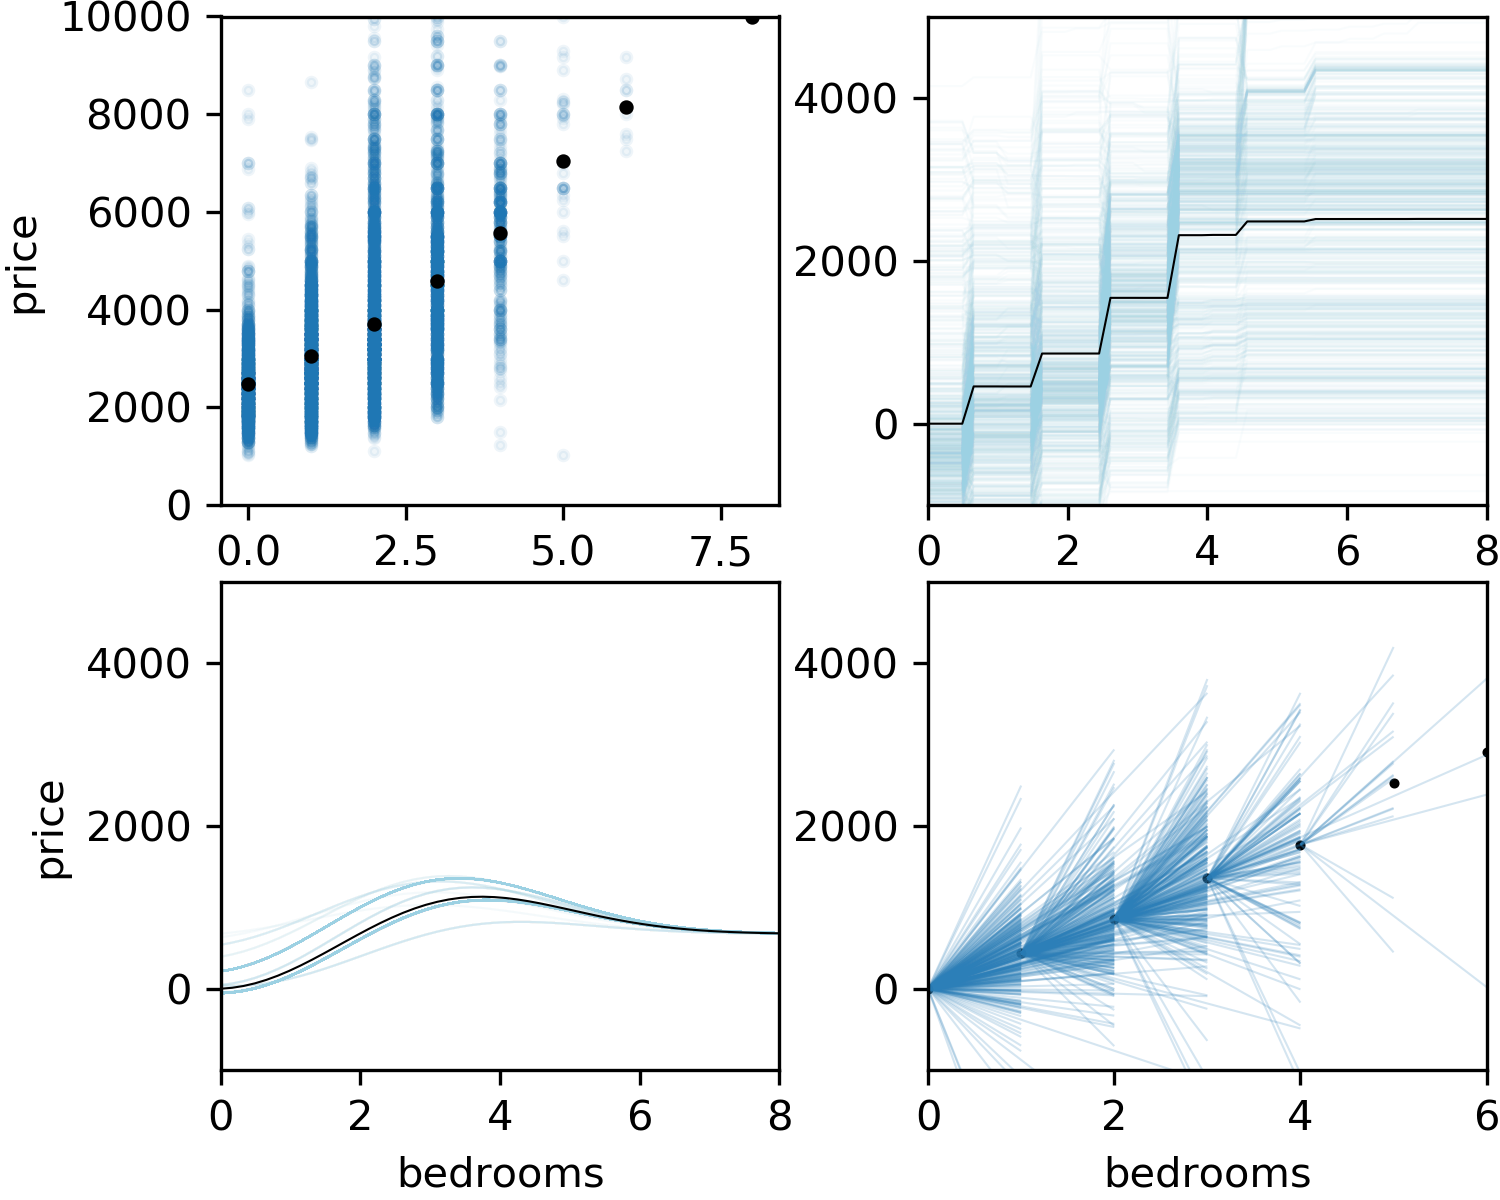
\includegraphics[scale=0.7]{images/bedrooms_vs_price.png}
\caption{{\bf  Marginal plot, PDP/ICE plot, and \spd{} plot of bedrooms versus rent price; sample size 9000 of 400k...}}
\label{fig:baths_price}
\end{center}
\end{figure}

\cut{The partial dependence plot broadly follows the marginal plot except for the prices of two and three bedrooms apartments, where it levels off. This is counterintuitive and exposes an issue with PD and ICE plots.} While PD and ICE plots are {\em model-agnostic}, they are not {\em model-independent} and are subject to the strengths and weaknesses of the model making predictions.  For example, Random Forests(tm) (RF) cannot extrapolate beyond their support range and this data set subset of 10,000 observations has very few apartments with more than 5 bedrooms.  (Note the lack of blue dots in that range of the marginal plot.) PD and ICE plots shift the bedrooms feature of all observations from 0 to 6, accepting less trustworthy predictions from the model in extreme ranges.   

Obtaining radically different PD and ICE plots for different underlying models is undesirable because users cannot distinguish between interesting target fluctuations and artifacts of their model choice. Consider \figref{fig:baths_price}(c) that shows the PD/ICE plot for the exact same data set but using a Support Vector Machine (SVM with $\gamma=1/p$). The SVM appears to have difficulty capturing the relationship between bedrooms and price evident from the marginal plot, which means PD and ICE plots derived from an SVM for this variable are not accurate; plots derived from high-bias models should not be trusted. At the very least, users of PD and ICE should compare plots derived from multiple models. 

\figref{fig:baths_price}(d) shows the partial dependence of rent on the number of bedrooms (as black dots) using the \spd{} approach described in this paper. The plot also depicts the density of data in the bedrooms/rent space by the number and location of lines, identifies the unique $x$ (bedrooms) values, and characterizes the variability of the slopes across $x$ by the spread of the line angles.

There are two remaining issues with PD plots associated with the relationship between features. First, as Friedman pointed out, PD plots are most accurate ``{\em when {\em [the model]} is dominated by low order interactions.}''  Feature interactions such as $x_1x_2$ are difficult to tease apart to obtain partial codependencies on just $x_1$ or $x_2$. (Feature $x_j^T = (x_{1j}, .., x_{Nj})$ is a column vector of the  $n \times p$ explanatory matrix ${\bf X}$). ICE plots address this issue by showing separate prediction curves for each observation as the feature of interest is moved through all possible values.  This not only shows the variation hidden by the PD average curve, but it depicts interaction relationships between the feature of interest and other features.

The second issue stems from a lack of independence between features.  In a nutshell, not every combination of codependent features is valid. Consider a five bedroom apartment with just one or even zero bathrooms or a four bathroom studio was no bedroom or an observation identified as male but also pregnant.  Because PD and ICE alter observations by shifting the feature of interest through all possible feature values, they run the risk of conjuring up nonsensical observations, and in our experience, features in real data sets are very often codependent to some degree. This problem can be mitigated by computing PD and ICE plots on groups of mutually-dependent or interacting features of interest. \todo{but could involve identifying subsets and computing lots of combinations and we still might want to know about a single contribution.}

\begin{figure}[htbp]
\begin{center}
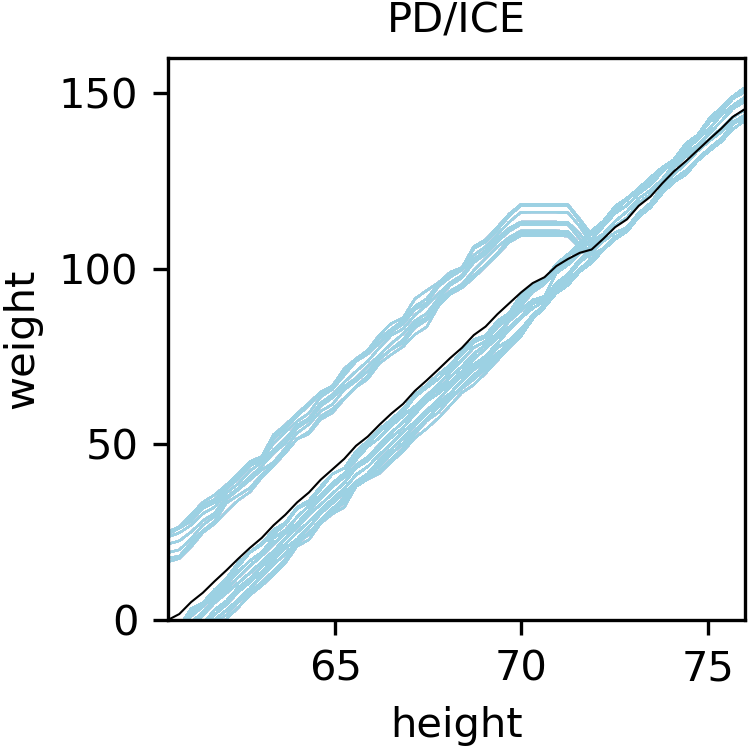
\includegraphics[scale=0.7]{images/height_vs_weight_pdp.png}
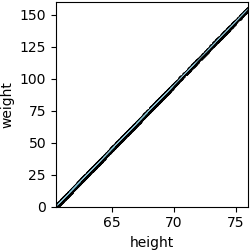
\includegraphics[scale=0.7]{images/height_vs_weight_stratpd.png}
\caption{{\bf  height and educ vs weight}}
\label{fig:height_vs_weight}
\end{center}
\end{figure}

To illustrate how variable codependencies result in misleading PD and ICE plots, consider a body weight data set with observations matching a person's characteristics to a weight in pounds. We discuss the data set details in \secref{sec:applications}, but for the moment, assume that women are slightly shorter on average and are 30 pounds heavier if pregnant. The PD/ICE plot in \figref{fig:height_vs_weight}(a) shows an inaccurate partial dependence where shorter people are slightly heavier per inch of height than those over about 72 inches. The blue ICE lines jump up significantly for shorter heights due to the codependence of $x_{sex}$ and $x_{pregnant}$ because PD and ICE conjure up pregnant males and ask the model to estimate their weight.  To be clear, the weight equation has no interaction term with $x_{height}$ and $x_{pregnant}$, but $x_{height}$ is codependent indirectly with $x_{pregnant}$ (via $x_{sex}$).  The \spd{} plot in \figref{fig:height_education_vs_weight}(b), on the other hand, is not confused by codependence and gives the true partial dependence of weight on height. 

\todo{needs a transition sentence here}

\section{A stratification approach}
{\color{red} JW - I haven't visited this section yet. I will update the notation but I was waiting for TP to resolve what method we use.}
\todo{this is probably the right time to say we simplify C to c single variable}
In a perfect world, supporting codependent and interacting features would be straightforward because we would know the actual function, $y = f(X)$ that precisely maps a feature vector $X$ to target value $y$. The partial derivative of $f(X)$ with respect to a single variable of interest $x_c$ describes how a unit change in $x_c$ affects $y$ for all $x_c$ values, treating all other variables as constants. Integrating the partial derivative $\frac{\partial}{\partial x_{c}} f(X)$ would yield a curve showing just $x_c$'s contribution to $y$. 

Even though $y = f(X)$ is unavailable, a linear regression model, $y = \hat{f}(X)$, provides the general trend of $y$ versus feature $x_c$ via regression coefficient $\beta_c$. For a unit change in $x_c$, $y$ increases or decreases by $\beta_c$, effectively canceling out or controlling for the other features, \xnc. There are two problems with the use of a global linear model, however.  First, a linear model might not be flexible enough to capture the relationship between all $(X,y)$ observation pairs. Coefficient $\beta_c$ is a constant and smooths over any local $y$ fluctuations across the entire range of $x_c$. Second, linear models require dummy variables to represent (and replace) categorical $x_c$ variables, therefore, regression coefficients would describe the relationship between the presence or absence of a single category and $y$, rather than $x_c$ and $y$.

Another simple but impractical approach stratifies a data set, grouping observations by all features except the feature of interest, $x_c$.  Let $G$ be a group of observations, identified by a set of row indices, where each observation has identical \xnc{} features. For a given $G$, the $\{(x_{ic},  y_i)\}_{i \in G}$ pairs then partially describe how $x_c$ affects $y$, all else being equal.  Regressing (without regularization) $y$ on $x_c$ for the observations in group $G$ yields an approximation of the slope of $y$, coefficient $\beta_G$, localized to the specific region of \xnc{} in group $G$; region $R_G = [min(x_{ic}), max(x_{ic})]_{i \in G}$. Because the $x_c$ regions from multiple groups could overlap, slope $\beta_R$ in any given $x_c$ region, $R$, would be the weighted average of all slope estimates covering that region: $\beta_R = \frac{1}{\Sigma_{G \in R} |G|}\Sigma_{G \in R}|G|\beta_G$. Together, the collection of regions and slopes, $\{(R, \beta_R)\}_{R \in x_c}$, would cover the full $x_c$ range and represent a good localized approximation of the partial derivative of the unknown $f(X)$ with respect to $x_c$.

Alas, this stratification approach works for two or three variables but breaks down for more variables because it is impractical to find groups of observations that are equal across so many variables.  Nonetheless, stratification is simple, well understood, and clearly isolates the effect of $x_c$ on $y$ from the other features, even in the presence of codependent and interacting features.  The only obstacle is a general and practical mechanism for stratifying observations with many variables, which leads us to the primary contribution of this paper.

\subsection{StratPD for numerical variables}

The key idea is to relax stratification so that it organizes observations into groups of similar rather than equal observations.  Our approach, called \spd, trains a decision tree regressor, $T$, as in \cite{CART} on $(x_{\overline{c}}, {\bf y})$ to stratify observations into regions of \xnc{} feature space with similar \xnc{} values. Each leaf in the tree, $L \in T$, represents a region of \xnc{} space and $(L_x, L_y)$ are the $x_c$ and $y$ observations associated with $L$. \spd{} then characterizes the relationship between $L_y$ and $L_x$ for each $L$ by (i) training another decision tree, $T'$, on $(L_x, L_y)$ to partition $x_c$ space into $(L'_x, L'_y)$ for each $L' \in T'$ and (ii) fitting a simple linear regressor to each subregion $(L'_x, L'_y)$.  The collection of $\beta_{L'}$ coefficients represent the localized slope across the $x_c$ space of $L$. Ignoring the $y$-intercepts removes the contribution of \xnc{} to $y$ in $L'$.

The regions of $x_c$ spanned by the various $\beta_{L'}$ generally overlap and the slope in any  region, $R$, is the weighted average of all $\beta_{L'}$ that overlap $R$:

\[
\beta_R = \frac{1}{\Sigma_{L' \in R} |L'|}\Sigma_{L' \in R}|L'|\beta_L'
\]

Slope $\beta_R$ is an estimate of the partial derivative across the region $R$, and so numerically integrating the partial derivatives across $x_c$ space gives a curve representing the contribution of $x_c$ to $y$.  Algorithm \ref{alg:StratPD} encodes the \spd{} process and the full Python 3 source code is available at {\small \url{https://github.com/parrt/stratx}}. \figref{fig:leaves} depicts the averaging and integration process.  

\begin{figure}[htbp]
\begin{center}
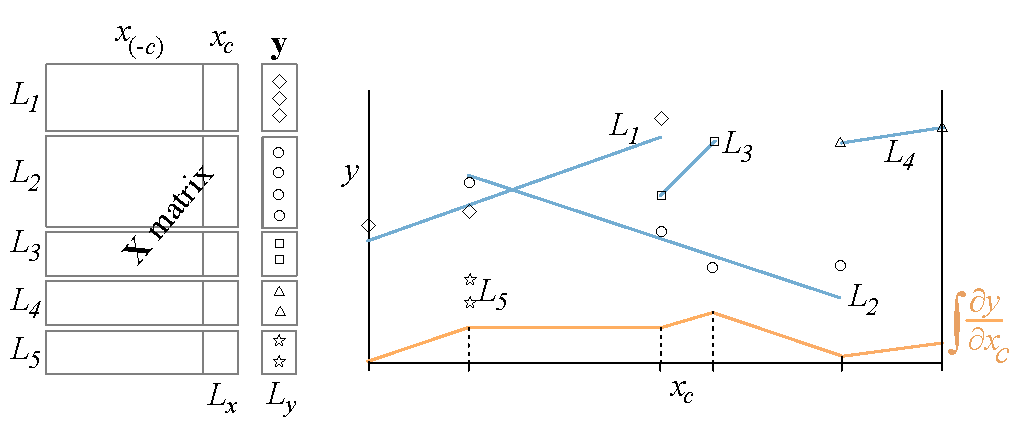
\includegraphics[scale=0.7]{images/leaves.pdf}
\caption{BLORT There are five leaves, $L_1 .. L_5$, with regression lines fit through leaf observations. The $x_c$ values in $L_5$ are identical so its infinite slope is ignored.}
\label{fig:leaves}
\end{center}
\end{figure}

\cut{
\spd{} trains a decision tree in the usual way but on $(x_{\overline{c}}, {\bf y})$ rather than $({\bf X}, {\bf y})$. Observations $(X_i, y_i)$ that end up in a tree leaf are, by definition, in the same region of \xnc{} feature space. Training greedily partitions feature space in order to minimize variance of $y_i$ within regions, which partitions feature space into tighter and tighter regions.  (The collection of variable inequality decision nodes along the path from from root to a leaf demarcates the region of feature space.) Tighter regions imply more similar \xnc{} values, which means $x_c$ is likely responsible for any variation in $y$; this likelihood decreases as the size of $L$ increases.  The training process must leave at least two samples per leaf in order to fit a localized linear model.  
}

Revisiting the \spd{} plot in \figref{fig:height_vs_weight}(d), derived from the apartment rent data set, each blue line represents a local slope $\beta_L'$ through the observations in $L'$ (which is a partition of $x_c$ space whose \xnc{} features are similar). Lines extend from the minimum to maximum $x_c$ value in $L'$.  Because we are interested in the relative contribution of $x_c$ to $y$, \spd{} plots use zero as a $y$-axis baseline. The black dots represent the integration of the partial derivative estimates up to and including each unique $x_c$ value (except the first $x_c$, whose integral value is 0). The partial derivative estimate at an $x_c$ value is the (weighted) average slope of the blue lines emanating from that value. \spd{} does not interpolate between $x_c$ points and so the plot shows dots not lines. 

Partial dependence through stratification also works for data sets with categorical variables in \xnc{}, given a suitable similarity measure between observations that supports categorical variables, but identifying an appropriate categorical similarity measure is a well-known issue.  Decision trees, however, support categorical variables easily and effectively by treating categories as unique integers. Observations with categorical variables that end up in the same leaf lie are likely to be similar. (\todo{cite breiman proximity matrix and p595 of ESL book}). Algorithm \ref{alg:StratPD}, therefore, works without modification for \xnc{} containing categorical variables. When the column of interest, $x_c$, is categorical, however, a new algorithm is required.

\subsection{CatStratPD for categorical variables}

The stratification approach can also capture how a categorical variable $x_c$ affects $y$, instead of just a single category at a time (if one were forced to dummy-encode $x_c$). As with \spd{}, the \cspd{} algorithm stratifies $\bf X$ into groups of similar \xnc{} features by training a decision tree regressor on $({\bf X}, {\bf y})$, yielding a collection of leaves. But, because categorical variables can be unordered nominal variables, the notion of $y$ slope is not meaningful between two categories. Instead of partitioning the $x_c$ space in each leaf $L$, \cspd{} groups leaf observations $(L_x, L_y)$ by the categories in $L_x$ and computes the average $L_y$ value per category.  Subtracting the mean of $L_y$ for a reference category from all category averages erases the $y$-contributions of \xnc{}, leaving a relative increase or decrease in $y$  for each category. Then, to get the overall contribution of $x_c$ to $y$ for category $cat$, \cspd{} averages the leaf contributions for $cat$ from all $L$ weighted by $|L|$. See Algorithm \ref{alg:CatStratPD}.

\figref{fig:state_vs_temp}(b) illustrates \cspd{} operating on a categorical variable, $x_{state}$, in a synthetic weather data set with data from four states over three years. Temperature data varies in sinusoidal fashion over the year with $N(-5,5)$ noise and different baseline temperatures per state, as the marginal plot in \figref{fig:state_vs_temp}(a) shows. To get the partial dependence of temperature on $x_{state}$, \spd{} stratifies by $x_{dayofyear}$ and $x_{year}$ then groups these similar time buckets by $x_{state}$ and computes the average temperature; each blue dot represents a leaf average. The overall temperature estimate per state is the average of those leaf averages, represented by a solid black dash. We use a strip plot to exhibit the variation and density of $y$ values per category. The \cspd{} plot accurately identifies the baseline temperature per state, as does the PD/ICE plot in \figref{fig:state_vs_temp}(c).

\begin{figure}[htbp]
\begin{center}
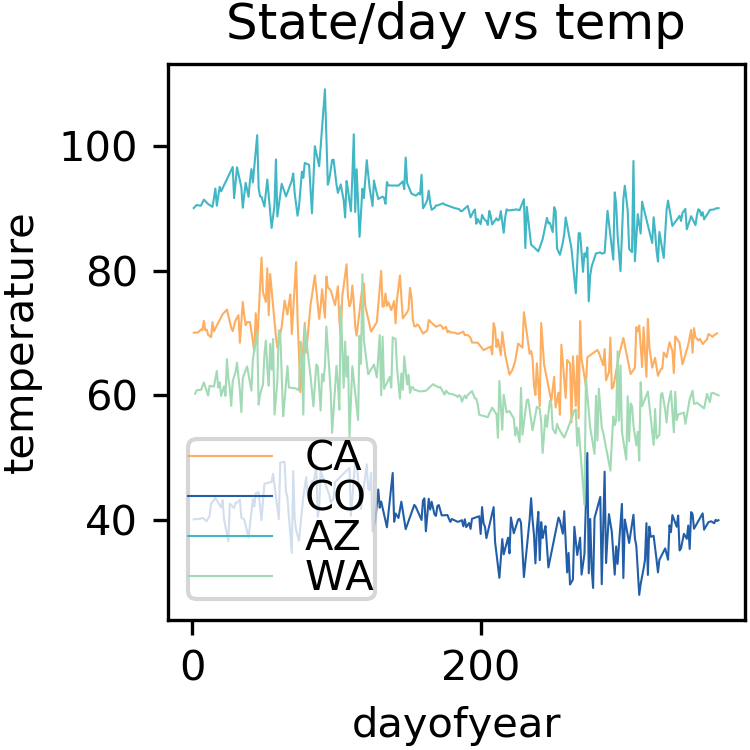
\includegraphics[scale=0.7]{images/dayofyear_vs_temp.png}
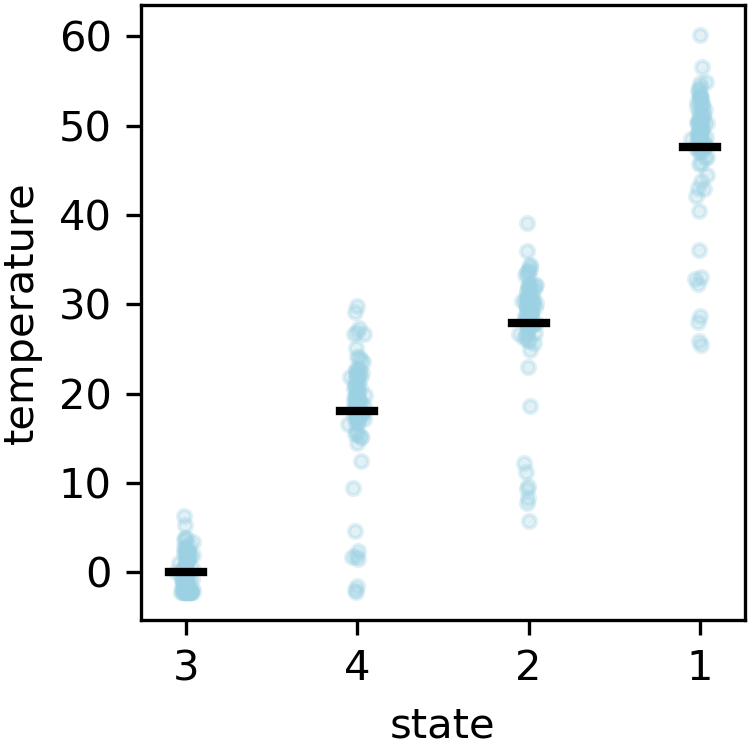
\includegraphics[scale=0.7]{images/state_vs_temp_stratpd.png}
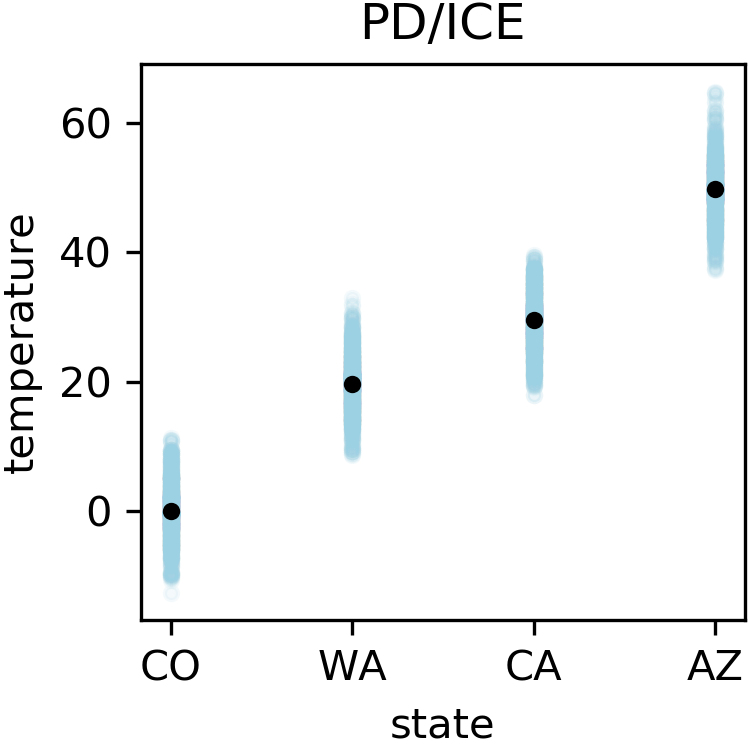
\includegraphics[scale=0.7]{images/state_vs_temp_pdp.png}
\caption{{\bf  state  vs temp}}
\label{fig:state_vs_temp}
\end{center}
\end{figure}

\subsection{Partitioning feature space with trees and forests}

Stratification of $(x_{\overline{c}}, y)$ into regions of similar observations is at the core of our approach so it's worth examining how \spd{} partitions feature space in more detail.  The goal is to examine $({\bf X}, {\bf y})$ for groups of extremely similar \xnc{} values so fluctuations in $y$ are due solely to changes in $x_c$, which yields a piece of the partial dependence of $y$ on $x_c$. \spd{} looks for similar observations because, beyond a few variables, it's not possible to stratify observations by equal \xnc{} values. 

Inventing a new partitioning strategy is unnecessary because decision trees already exist that can tesselate \xnc{} feature space into small hypervolumes of similar observations. If a hypervolume is tight enough, then \xnc{} values are very similar and the slope of a regression line through $(Lx, Ly)$ is a good estimate of the partial derivative of $\frac{\partial y}{\partial x_{c}}$ in that region.  If the volume for leaf $L$ is too large, then \xnc{} observations in $L$ are not similar enough to conclude that changes in $y$ are due to $x_c$ alone. By default, our Python implementation of \spd{} creates decision trees with at least two observations per leaf, but depending on $y$, leaf size is unbounded. As discussed in \secref{sec:patho}, large leaves should themselves be partitioned into a collection of smaller leaves using another decision tree, but this time training and partitioning $x_c$ rather than \xnc{}.  Because training occurs on \xnc{}, leaf observations can have overlapping $x_c$ regions so, for a given range $R$, \spd{} averages the $\beta_L$ slopes for all $L \in R$ giving $\beta_R$.  The partial derivative across the entire $x_c$ range is the sorted collection of $\beta_R$.

Decision trees are known to overfit like mad, which was the impetus for the invention of Random Forests(tm) (RF) \cite{RF}.  \spd's use of decision trees rather than RFs, therefore, seems an odd choice. Indeed, using RFs was our initial approach and the \spd{} source code still supports them. (The only change to the algorithm described in this paper is to iterate over all leaves from all trees, rather than the leaves of a single tree, to collect $\beta_L$ slopes.)  Decision trees are sufficient for partial dependence, however, because the goal is to understand the population described by the training set, not to make predictions; that is what models are for. 

To reduce overfitting, RFs bootstrap and select split variables from a subset of all variables in order to create uncorrelated trees. But, that means increasing bias to some degree because each tree is trained on roughly 2/3 of the training data and without considering some of the variables. Because our goal is to group together {\em all} observations that are similar in {\em all} \xnc{} variables, it is counterproductive to bootstrap and select variables from a subset. Because partial dependence is meant to explore existing $(\bf X, y)$ data rather than future data, there's no point in sacrificing accuracy for the sake of generality. 

For the data sets we examined during the preparation of this paper, moving from a decision tree to a random forest of various sizes did not affect the partial dependence results; \figref{fig:weight_ntrees} and \figref{fig:rent_ntrees} show some typical results. The integrated partial derivative curves identified by the black dots do not change as the number of trees increases from left to right.  In one simulation run for the rent data set, we did see a difference in the partial dependence dots for an extreme value of $x_{bedrooms}$ with very few $y$ values, but it's unclear which plot is correct for this real data set. (The answer is unclear because the true partial dependence for a variable of an unknown function is unknown.)

The blue lines representing piecewise partial derivative estimates increase in number as the number of partitions (leaves) increases.  Note that the variance of the partial derivative estimates is wider for RFs than for a single decision tree. This is expected because the decision tree leaves contain all observations in a feature space hypervolume and so the estimate will be less biased; RF leaves have at most 2/3, the bootstrapping population size estimate, of the observations for the same hypervolume. The education versus weight plots in \figref{fig:weight_ntrees} illustrate this most clearly. The blue ``cone'' around the partial dependence dots widens as the number of trees increases.  

Increasing the number of trees does not improve accuracy and increases the time complexity linearly in the number of trees, which is roughly what we see in practice.  For example, using a single decision tree to partition a 9000-observation rent data set sample and generate a plot takes 1.5s on our 4.0Ghz processor but about 50s for 30 trees (first row, far right of \figref{fig:rent_ntrees}). \todo{seems less accuarate with bootstrap}

\begin{figure}[htbp]
\begin{center}
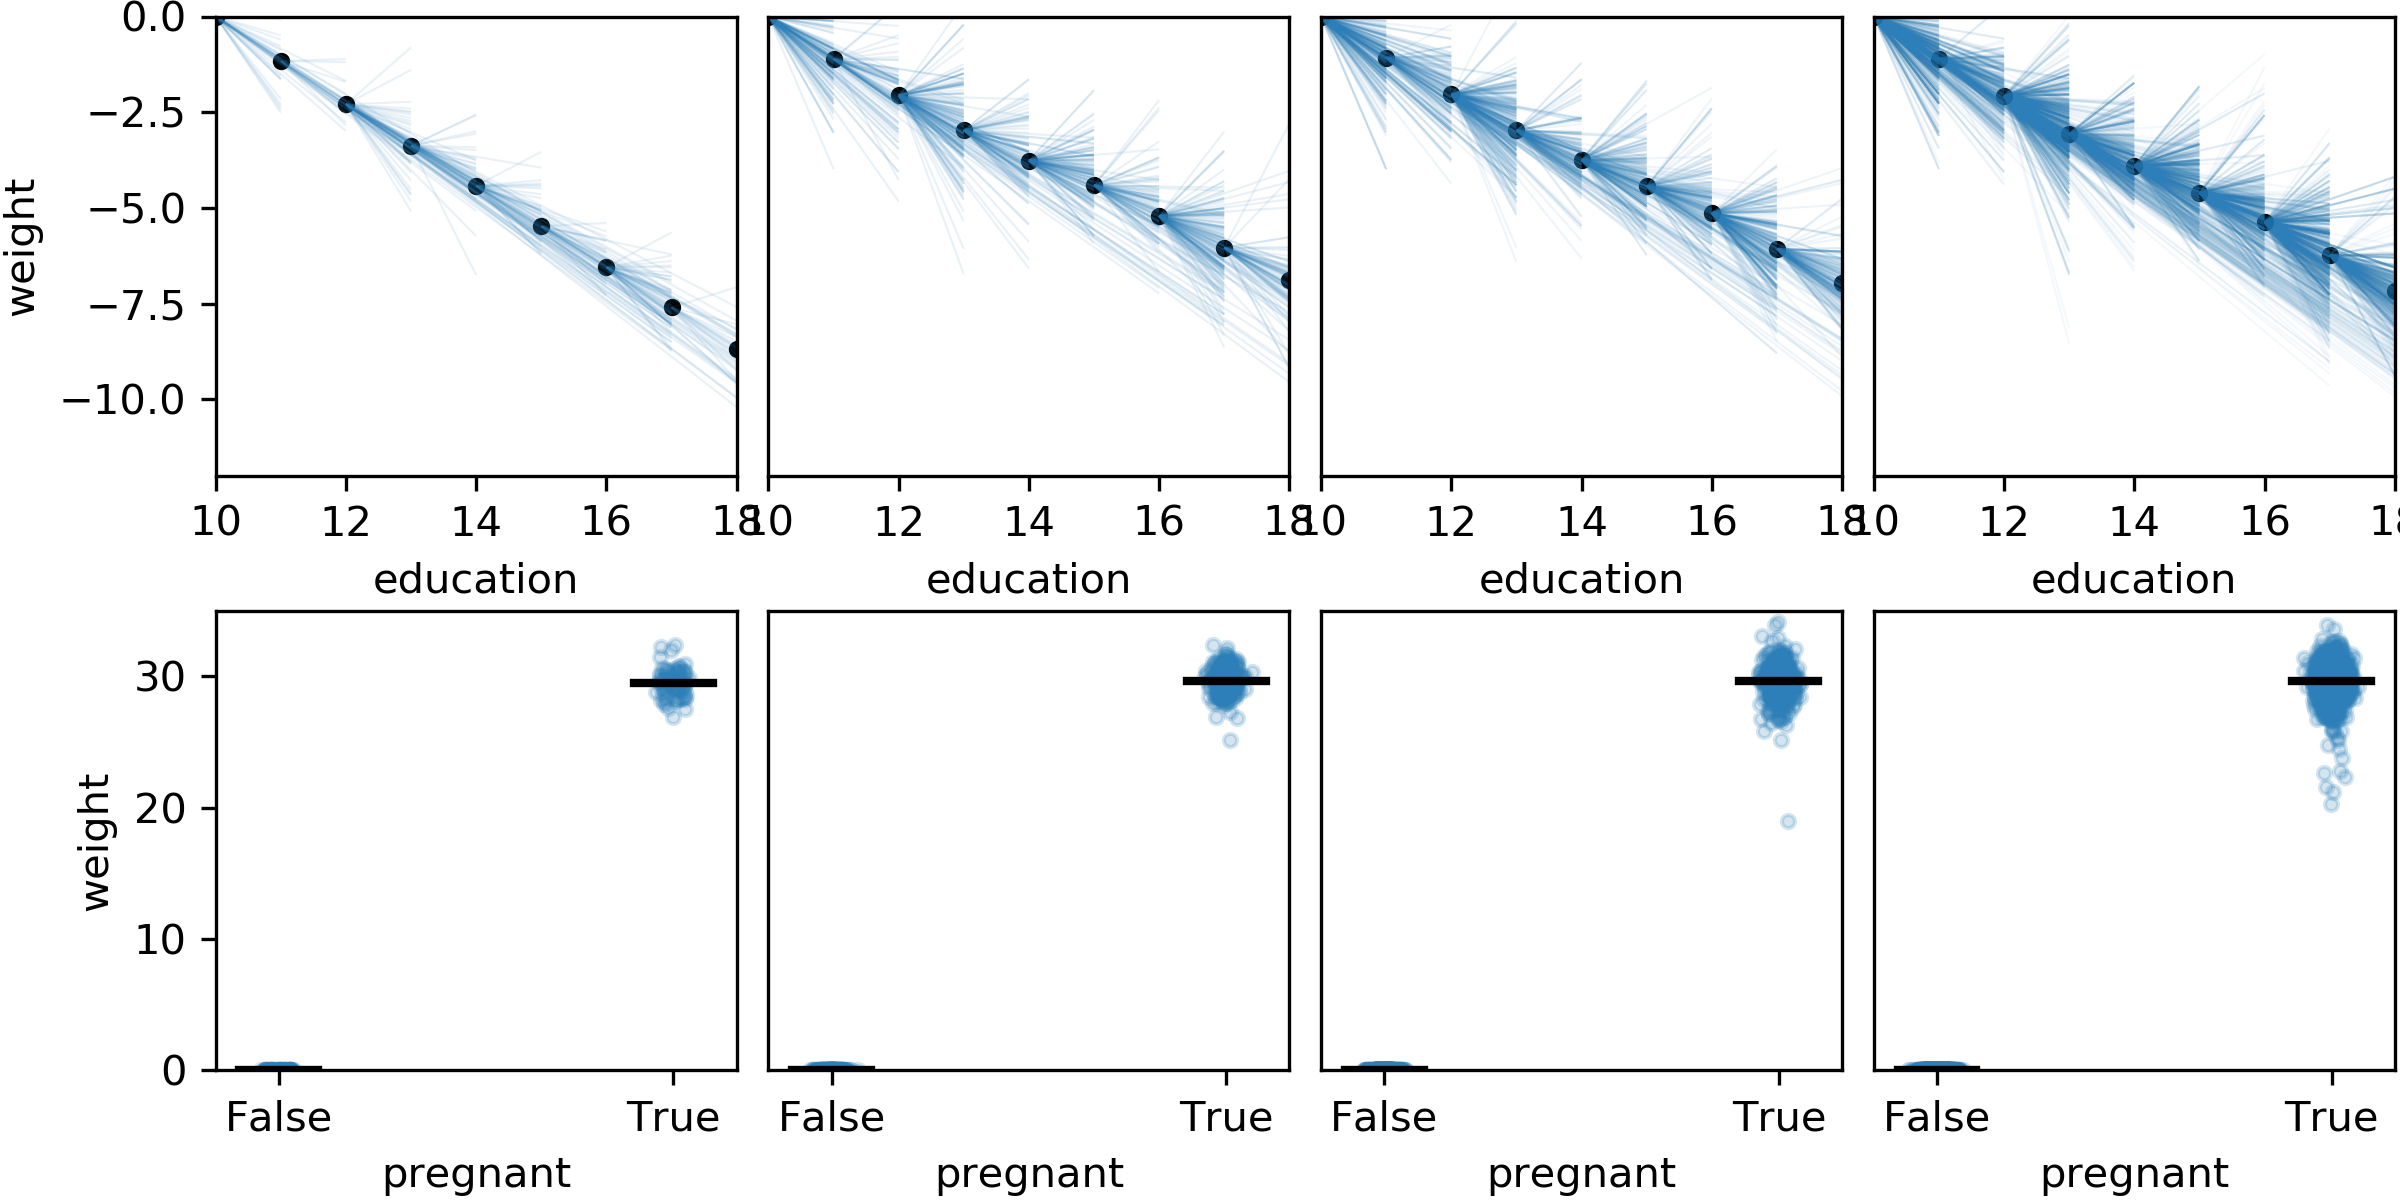
\includegraphics[scale=0.5]{images/height_pregnant_vs_weight_ntrees.png}
\caption{{\bf  weight ntrees 1, 5, 10, 30 trees}}
\label{fig:weight_ntrees}
\end{center}
\end{figure}

\begin{figure}[htbp]
\begin{center}
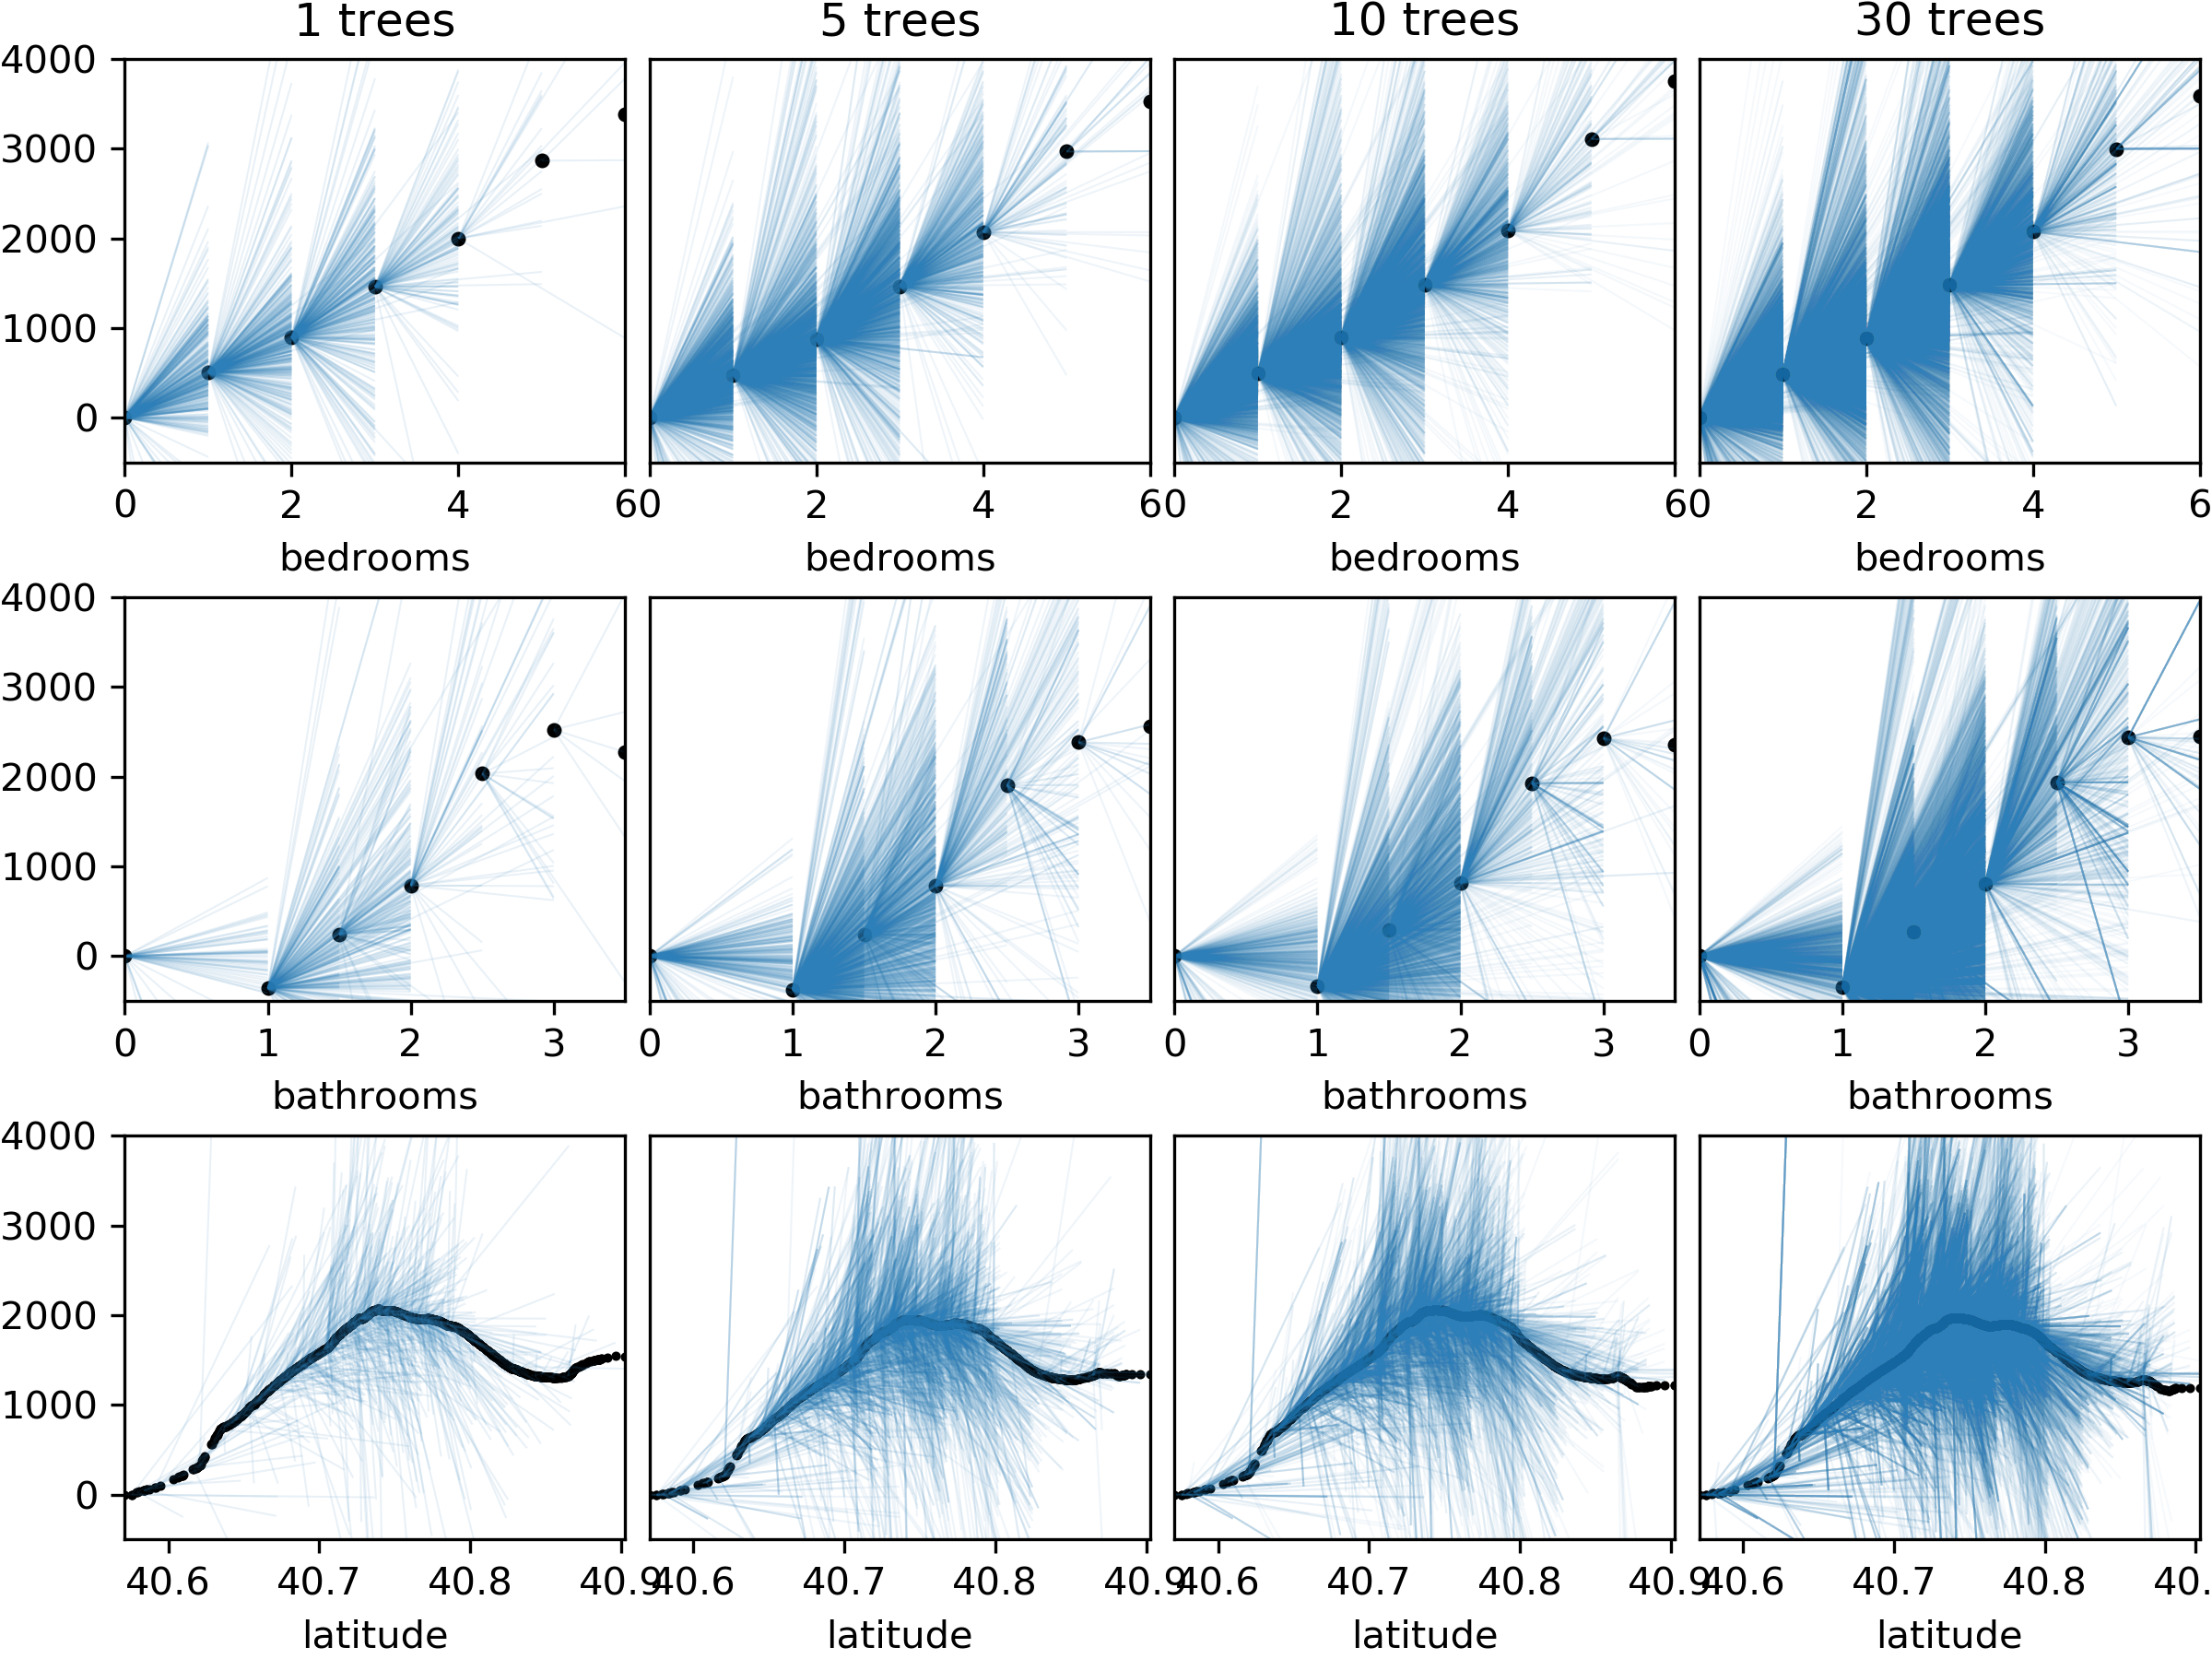
\includegraphics[scale=0.5]{images/rent_ntrees.png}
\caption{{\bf  rent ntrees 1, 5, 10, 30 trees}}
\label{fig:rent_ntrees}
\end{center}
\end{figure}

Decision trees choose feature space hypervolumes that minimize the variance in $y$, but $y$ is technically not needed to partition \xnc{} into similar regions. \cite{RFunsup} described how to use random forests in an unsupervised fashion by considering the original $\bf X$ matrix as class 1 and a synthesized $\bf X'$ as class 2, which works equally well for decision trees. $\bf X'$ is just $\bf X$ with each $x_j$ column permuted, effectively sampling from the $x_j$'s marginal distributions. \figref{fig:rent_weight_unsup} shows typical results from three variables from the rent data set and two variables from the synthesized weight data set.  The left column shows unsupervised partitioning of $\bf X$ and the right column shows the usual supervised partitioning with $(\bf X, y)$. The results are very similar but the variance of the partial derivative estimates for the unsupervised case appears to be a bit wider. The \cspd{} unsupervised and supervised plots for categorical variable $x_{pregnant}$ in \figref{fig:rent_weight_unsup}(b) are virtually indistinguishable to the eye. 

\figref{fig:boston_unsup} illustrates a case where unsupervised partitioning is less stable, sometimes giving obviously incorrect results: AGE versus MEDV (median house value) from the well-known Boston housing data set \todo{ref ICE's use in their paper}. The top row shows the unsupervised then supervised \spd{} plots, while the bottom left is the traditional AGE versus MEDV marginal plot and the bottom right is the PD/ICE plot. We tried simulations using a random forest with 10 trees, but the Boston unsupervised \spd{} plot was still erratic. The failure could be from the small size (506 observations), but in the end, there's no reason to perform unsupervised partitioning when $y$ is always available. (Partial dependence makes no sense without $y$.) 

The point is that partitioning \xnc{}  with a decision tree is more about $\bf X$ than $\bf y$, which strengthens our claim of model-independence. \spd{} does not rely on a user's model, never makes predictions from internal models, and can even get away with partitioning feature space without $\bf y$.

\begin{figure}[htbp]
\begin{center}
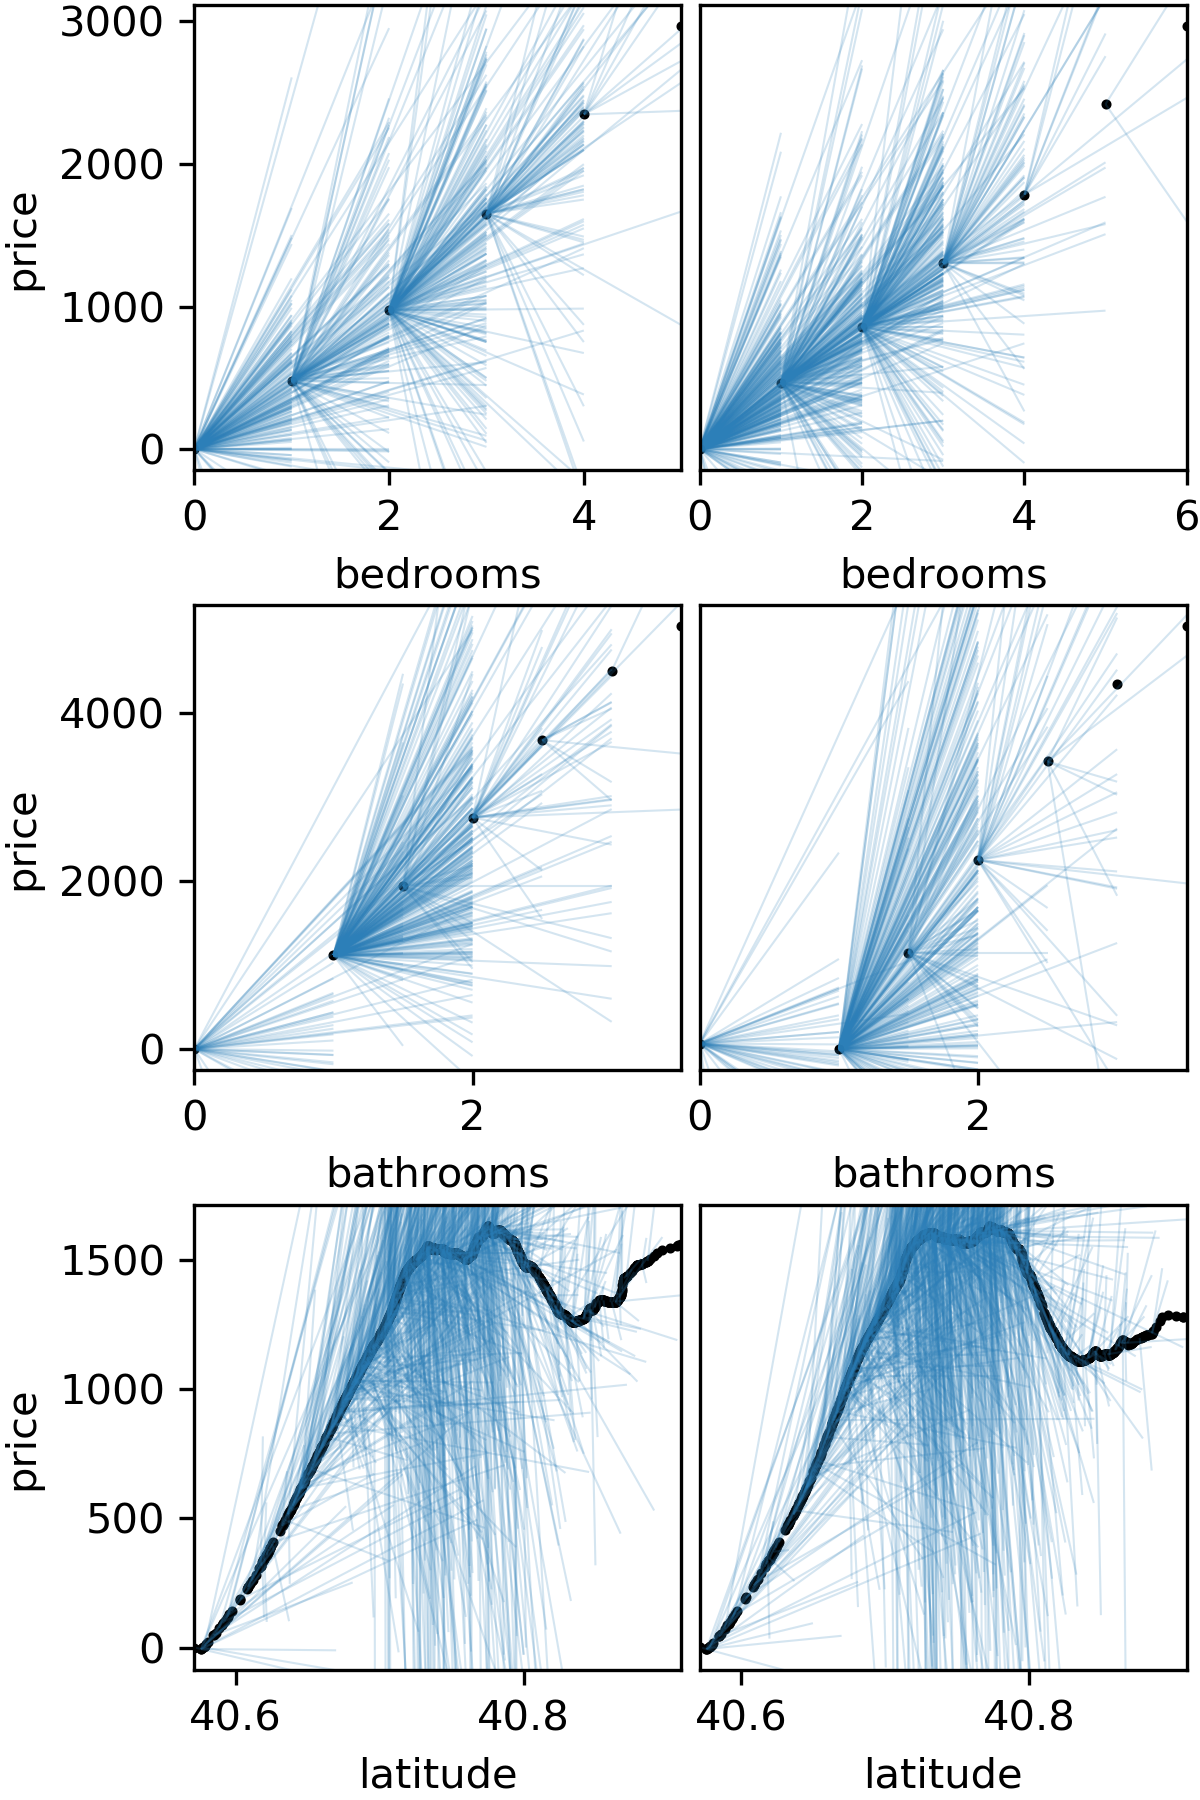
\includegraphics[scale=0.7]{images/rent_unsup.png}
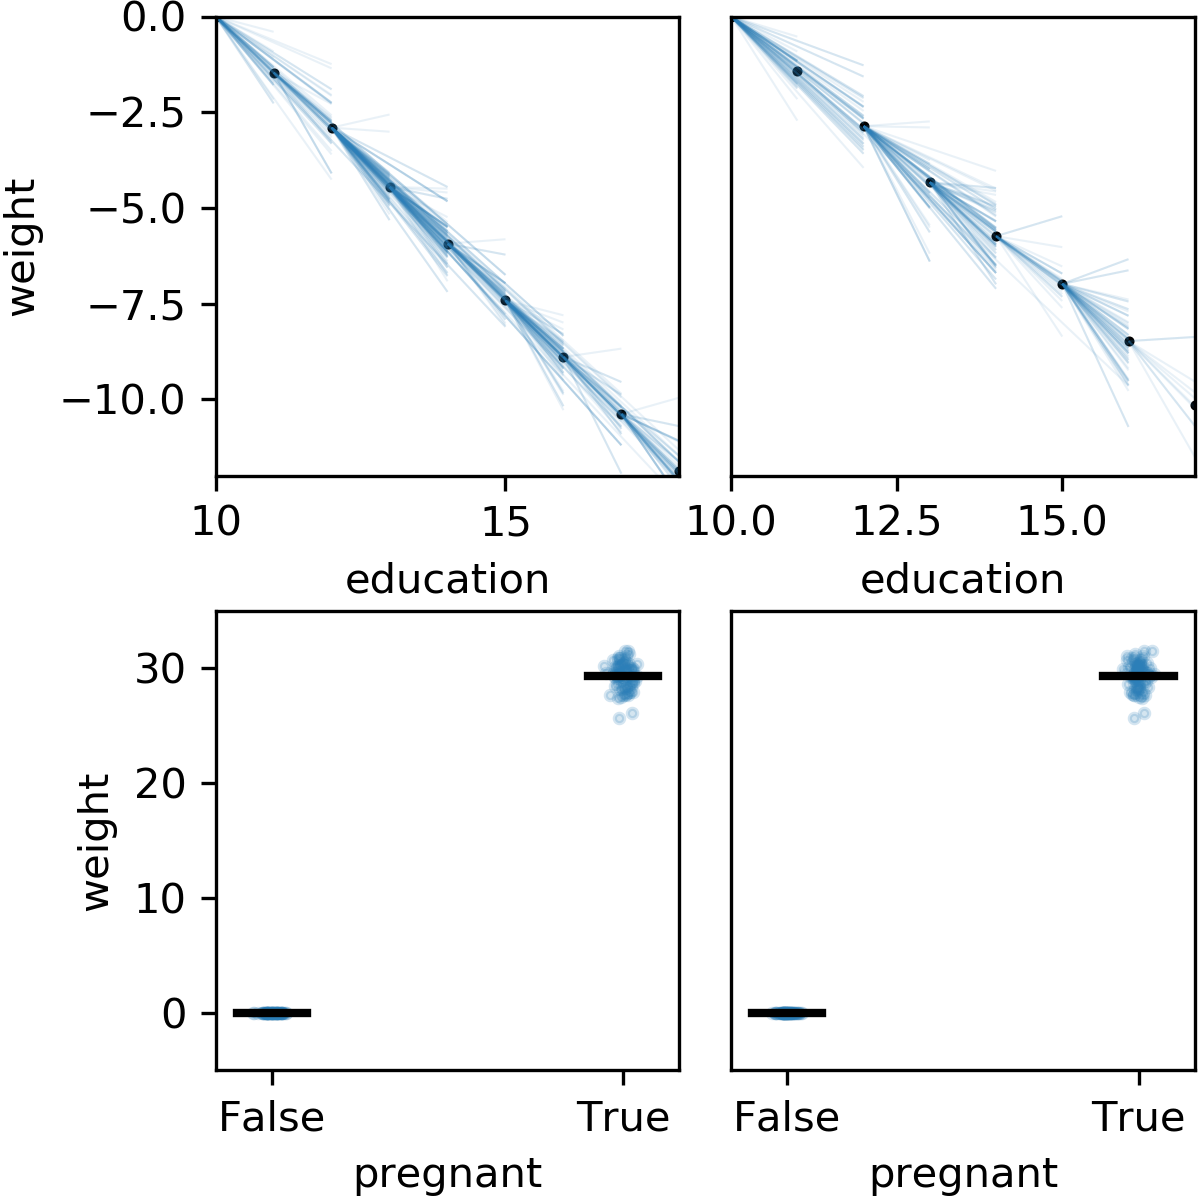
\includegraphics[scale=0.7]{images/weight_unsup.png}
\caption{{\bf  rent and weight unsupervised}}
\label{fig:rent_weight_unsup}
\end{center}
\end{figure}

\begin{figure}[htbp]
\begin{center}
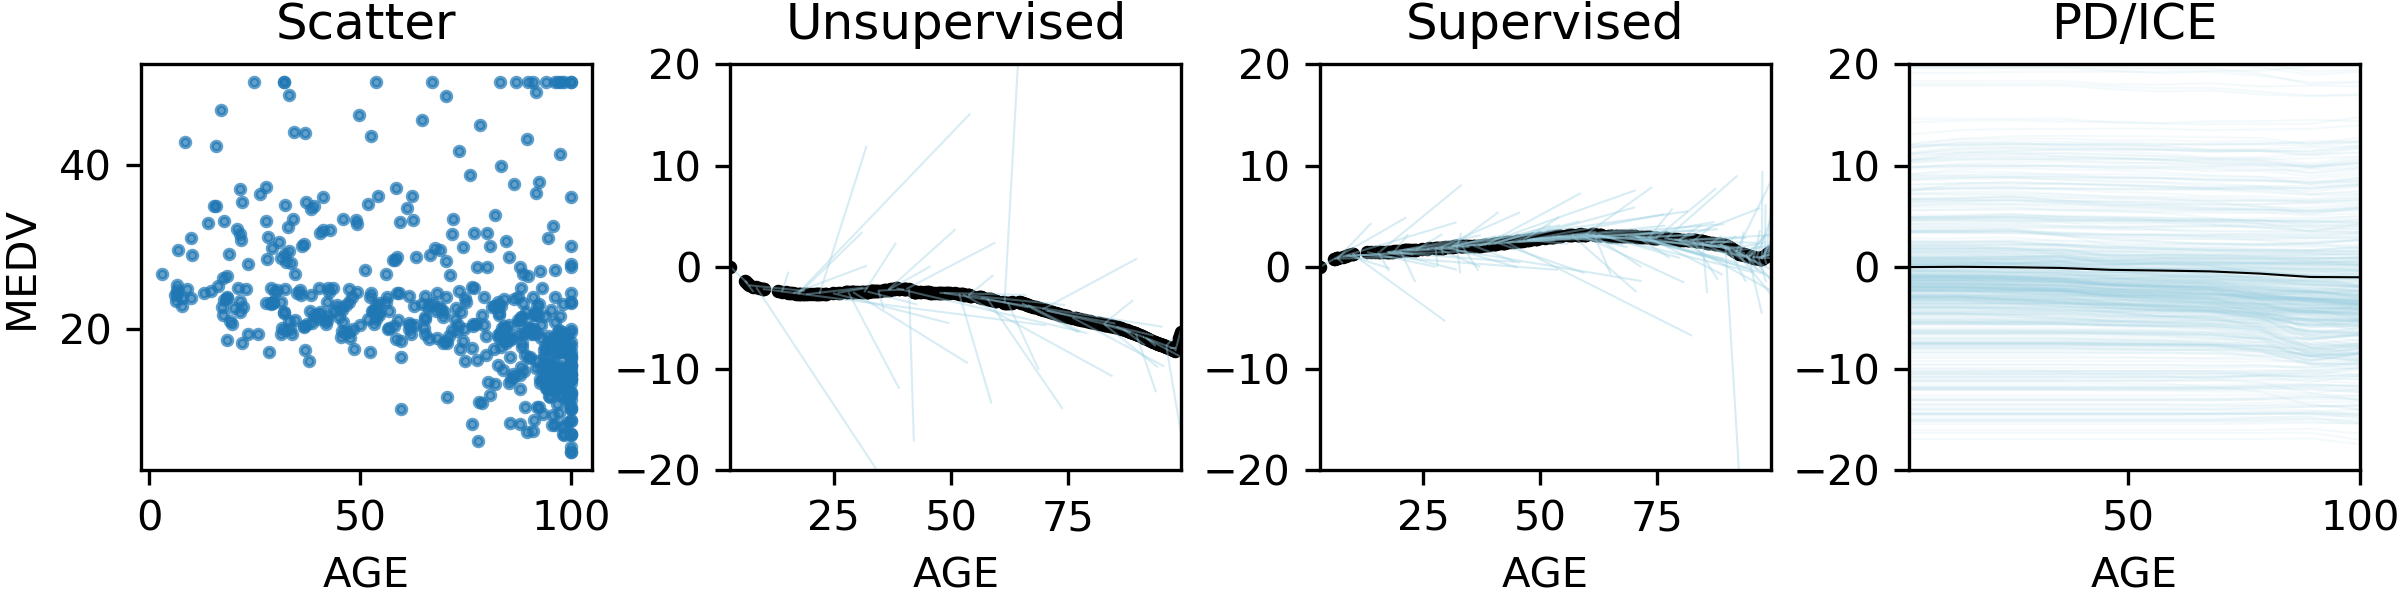
\includegraphics[scale=0.7]{images/boston_unsup.png}
\caption{{\bf   Boston unsup}}
\label{fig:boston_unsup}
\end{center}
\end{figure}

\todo{\spd{} degenerates to a simple marginal plot if training yields a tree with a single leaf node containing all of \xnc{}. where does this go?}

\todo{is this where we put edge cases of hyper parameters, num cols, etc? ref future experiment section. what are degenerate cases? approximation error.}

\section{Related Work}\label{sec:related}

We now describe related model interpretability methods, including ICE and PDP, in detail. The starting point for any marginal dependence method is to assume that there is some unknown model $f(\cdot)$ that describes the relationship between the features of interest $X$ and the response $y$:
\vskip -1pc
$${y} = f({X}).$$  PDP and ICE each rely on the practitioner first estimating $f$ with some machine learning model before estimating partial effects. Given a fitted model $\widehat{f}$, PDP and ICE estimate the partial effect between $x_C$ and the fitted model $\widehat{f}$. 

PDP seeks to estimate the partial dependence function $\widehat{f}^{PDP}_C(x_C)$ given by

\begin{equation*}\label{eq:PDP} \widehat{f}^{PDP}_C(x_C): = \mathbb{E}_{\overline{C}}\left[\widehat{f}({X})\right] = \int \widehat{f}({X}) d\mathbb{P}(X_{\overline{C}}).\end{equation*}


The function $\widehat{f}_C(x_C)$ describes the average marginal effect that the features $X_C$ has on the prediction $\widehat{f}$. The partial dependence of $X_C$ is a global representation of variable dependence and averages over any heterogeneous relationships between $\mathbf{y}$ and $x_C$. 

The individual conditional expectation (ICE) plot from \cite{ICE} is a local method which estimates the partial dependence of the prediction $\widehat{f}({X})$ on $x_C$ across individual observations. Suppose that $(X_{C_i}, X_{\overline{C}_i})$ are the values of the $i$th row of $\mathbf{X}$. For each $i$, the ICE plot produces a curve from the fitted model over all values of $X_C$ while holding $x_{\overline{C}_i}$ fixed. In particular, for observation $i$ the following curve is plotted $\widehat{f}^{(i)}_C = \widehat{f}((\{X_{C_i}\}_{i = 1}^n, X_{\overline{C}_i}))$. Unlike PDP, ICE can be used to  identify heterogeneous relationships between the fitted model and the features of interest $X_C$. By construction, the PDP curve for a variable $X_C$ is the average over all ICE curves for that variable. In practice, typically both ICE and PDP are used to describe the partial dependence of $\mathbf{y}$ on $X_C$.

An important limitation of PDP and ICE is that they require independence of the features in $\mathbf{X}$. This is rarely the case in practice, and in such situations these plots lead to faulty inference and misinterpretation (see \cite{apley2016visualizing} for a discussion). \cite{apley2016visualizing} introduced the accumulated local effects (ALE) strategy to overcome the independence limitation. The ALE plot is an average partial dependence of $X_C$ on $\widehat{f}$ that is calculated through the accumulation of local changes in the prediction for small windows of $X_C$. Local changes are measured as gradients of $\widehat{f}$ with respect to $X_C$ while $X_{\overline{C}}$ is held fixed. Although the ALE plot is unbiased in the presence of codependent features, it still has some disadvantages. Unlike \spd{}, ALE is not directly suitable for categorical variables as an ordering of each variable is needed for the calculation of gradients of $\widehat{f}$. Furthermore, the user must determine the number of intervals to use for calculating an ALE plot, and there is no general advice on how to do this.

%LIME
\cite{ribeiro2016should} proposed the local interpretable model-agnostic explanations (LIME) method as a strategy to interpret machine learning predictions. For a prediction of interest, LIME learns an interpretable model, on a small neighborhood of data around that prediction that explains the relationship between variables and the response locally. In contrast to \spd{}, LIME is used to create local interpretable models for each prediction; however, it does not directly assess the partial dependence of the response on a subset of variables. Like LIME, \spd{} also relies upon local interpretable models; however, \spd{} does this to explain partial dependence relationships rather than correlative relationships between the response and features. 

%Shapley
The Shapley strategy, introduced in \cite{lundberg2016unexpected}, is a permutation-based method for estimating the relationship between ${y}$ and a variable $X_C$ through a fitted model $\widehat{f}$. In this method, the marginal effect of $X_C$ is represented by the Shapely value, which is the average change in the prediction made from the original data $\widehat{f}$ and the prediction made when all other variables $X_{\overline{C}}$ have been randomly shuffled in the dataset. The permuting of $X_{\overline{C}}$ is repeated many times and the average Shapely value is reported as the importance. Like PDP, ICE, and ALE, the Shapely strategy is also dependent on the machine learning model fitted. Further, like any permutation method, this strategy can suffer from nonsensical observations due to the permuting of $X_{\overline{C}}$, which are subsequently incorporated in the estimated dependence. This is especially problematic in the case of highly correlated features. Finally, a major disadvantage of the Shapely strategy is its computational complexity due to repeated permutations. 

{\color{red} Add partial effects and LOESS?}

{\color{red} Causality?}

% $$\widehat{f}^{ALE}_C(x_C): = \int_{z_o}^{x_C}\mathbb{E}_{\overline{C}|C}\left[\dfrac{\partial \widehat{f}(\mathbf{X})}{\partial x_C} | x_C = z\right] dz = \int_{z_o}^{x_C}\int_{x_{\overline{C}}} \dfrac{\partial \widehat{f}(\mathbf{X})}{\partial x_C} \mathbb{P}(x | z)dxdz, $$
%Put a plot of ICE, PDP, and ALE, econometric stuff, 
% \noindent where $\mathbb{P}(x | z)$ is the conditional distribution of $x_{\overline{C}}$ given $x_C$.


% To summarize the hazards of PD and ICE plots, (i) both are strongly affected by the model chosen by the user, (ii) to obtain accurate plots, PD and ICE rely on the accuracy of the underlying model, which might sacrifice local accuracy to minimize some global loss function. Both plots display model prediction results rather than the data itself. (iii) The potentially inaccurate model feeds off of potentially nonsensical, synthesized observations arising from variable codependencies. What we need is an accurate mechanism that does not rely on, nor make predictions from, a user's model and a mechanism that does not assume mutually independent features.


% PDP math shows that features added or multiplied times the remaining F approximation completely describe the partial dependence; I assume that means that interactions are not a problem.

% Most importantly, \spd{} is model-independent in the sense that it does not expect nor rely on a user's model trained on $({\bf X}, {\bf y})$.  \spd{} does, of course, use models internally: a random forest for stratification and multiple linear models for estimating local partial derivatives.  The biggest difference is that \spd{} does not use predictions from any these models, which means prediction accuracy is irrelevant.  (\todo{refer to unsupervised learning trick}.)  In contrast, PD and ICE rely completely on the model supplied by the user and its accuracy.  Some implementations lay a grid across $x_c$'s range and, therefore, potentially make predictions based upon values not present in $x_c$. Also, as discussed, PD and ICE potentially conjure up nonsensical ${\bf }_i$ feature vectors, due to codependencies, and incorporate resulting predictions into plots.
%
%
%
%
% \spd{} was designed to support codependent features, which violates an assumption of PD and ICE. While ICE exposes variable interactions, it is still susceptible to variable codependencies causing misleading plots.
%
% do we need to talk about LIME? http://arxiv.org/pdf/1602.04938v1.pdf ?Why Should I Trust You?? Explaining the Predictions of Any Classifier.
%
% there are other ways to stratify X, such as quartiles or binning of some kind but we have to choose the bins or the similarity measure.
%
% talk about the derivative plot being meaningless in ICE.  they are smoothing and then taking the derivative of suspicious data.
%
% propensity stuff James mentioned
%
% talk about how we do not presume independence of features
 
% This python package seems to do PDP, LIME etc... https://github.com/oracle/Skater

\section{Experimental Results}\label{sec:applications}

We begin by reproducing graphs from \cite{ICE} big X from ICE, additivity from PD/ICE

bulldozer  just features 'ModelID', 'YearMade', 'MachineHoursCurrentMeter'; speculate that there is codependents between model and year made and machine hours. one would expect a log law for the model ID as some are much more expensive than the others. we would also expect a log law for the year made. not sure why ice is getting such a high value for machine hours.  note that machine hours of zero is probably missing or don't want to say so we deleted; less than 1950 deleted also.  sample of 10,000.


effect of noise columns (more data? change hyper parameters?), effect of hyper parameter changes
                 {\tt min\_samples\_leaf\_partition}=10,
                 {\tt min\_samples\_leaf\_piecewise}=.20,

effect of duplicated columns (need trees with less than max features)
	ntrees, max features, bootstrap

pathological case; sinewave

integer variables; currently the category stuff is messed up so the bathrooms don't look right; it should start at zero not one.

cars: show smoother and fits better

--------------------

Q: how does noisy columns affect ability to identify data features? does adding more data help?

Q: how does adding a noise column affect...?

Q: how does duplicating a column affect the ability to identify features? Does it depend on the data set and which feature?

Q: what are the hyper parameters and what advice do we have for setting them?

Note: if integer x then sometimes all y values fall directly on that x and no deriv can be computed.  must crank up number of samples and hires leaf size? i'm seeing num bedrooms in leaf as 0,1,2 but only get one piecewise line due to partitioning (all values are for single num bed value so ignored). sometimes even no piecewise lines if min\_samples\_leaf\_hires is low like 0.1

\begin{figure}[htbp]
\begin{center}
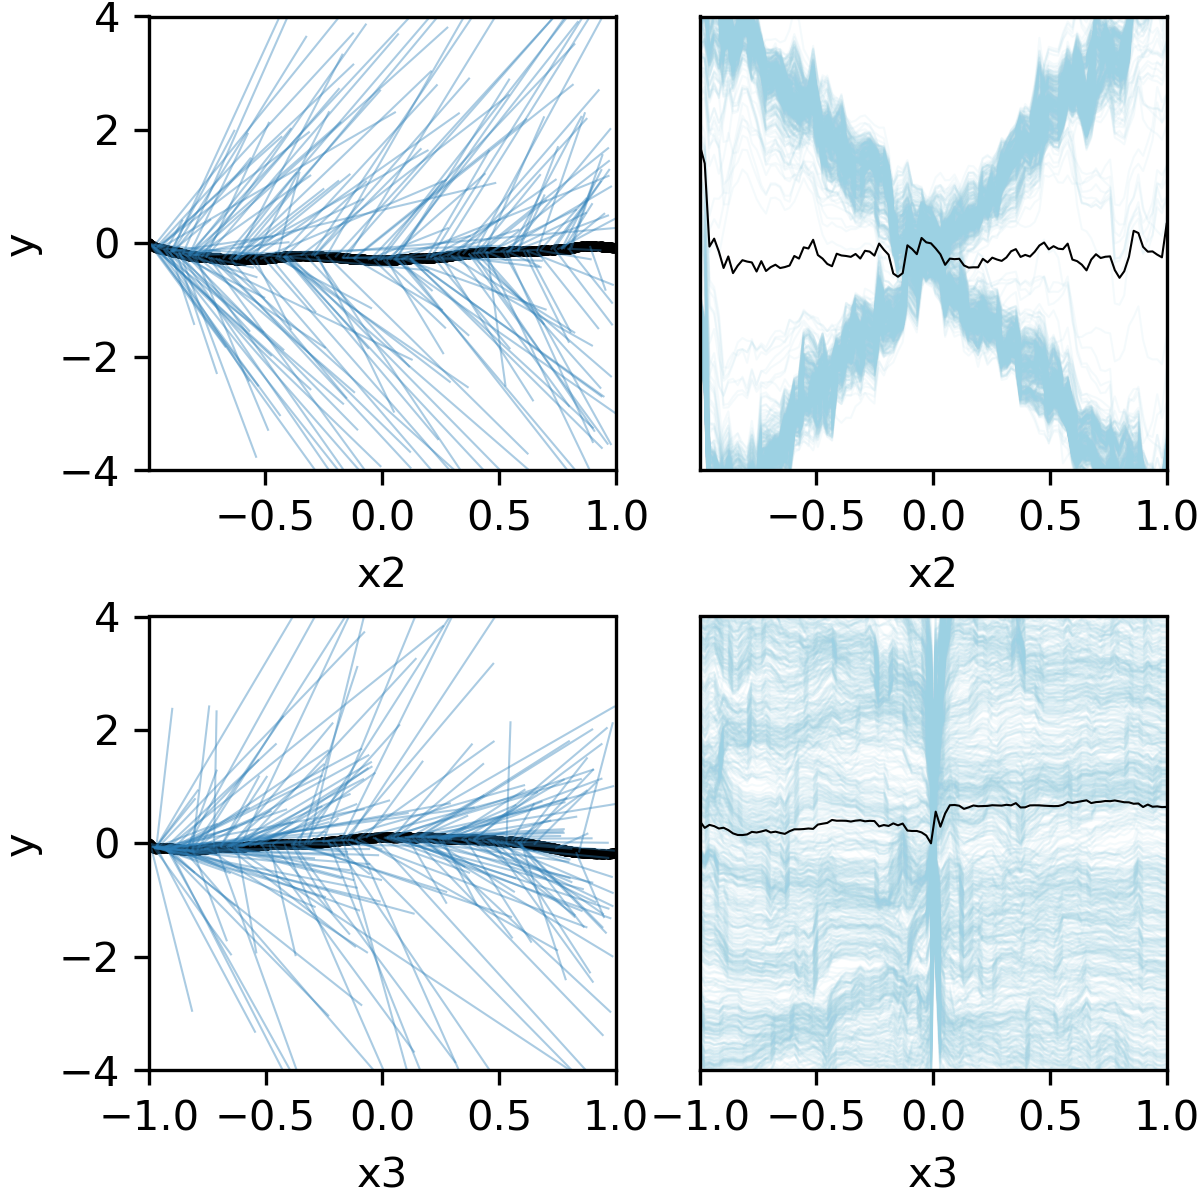
\includegraphics[scale=0.7]{images/bigx.png}
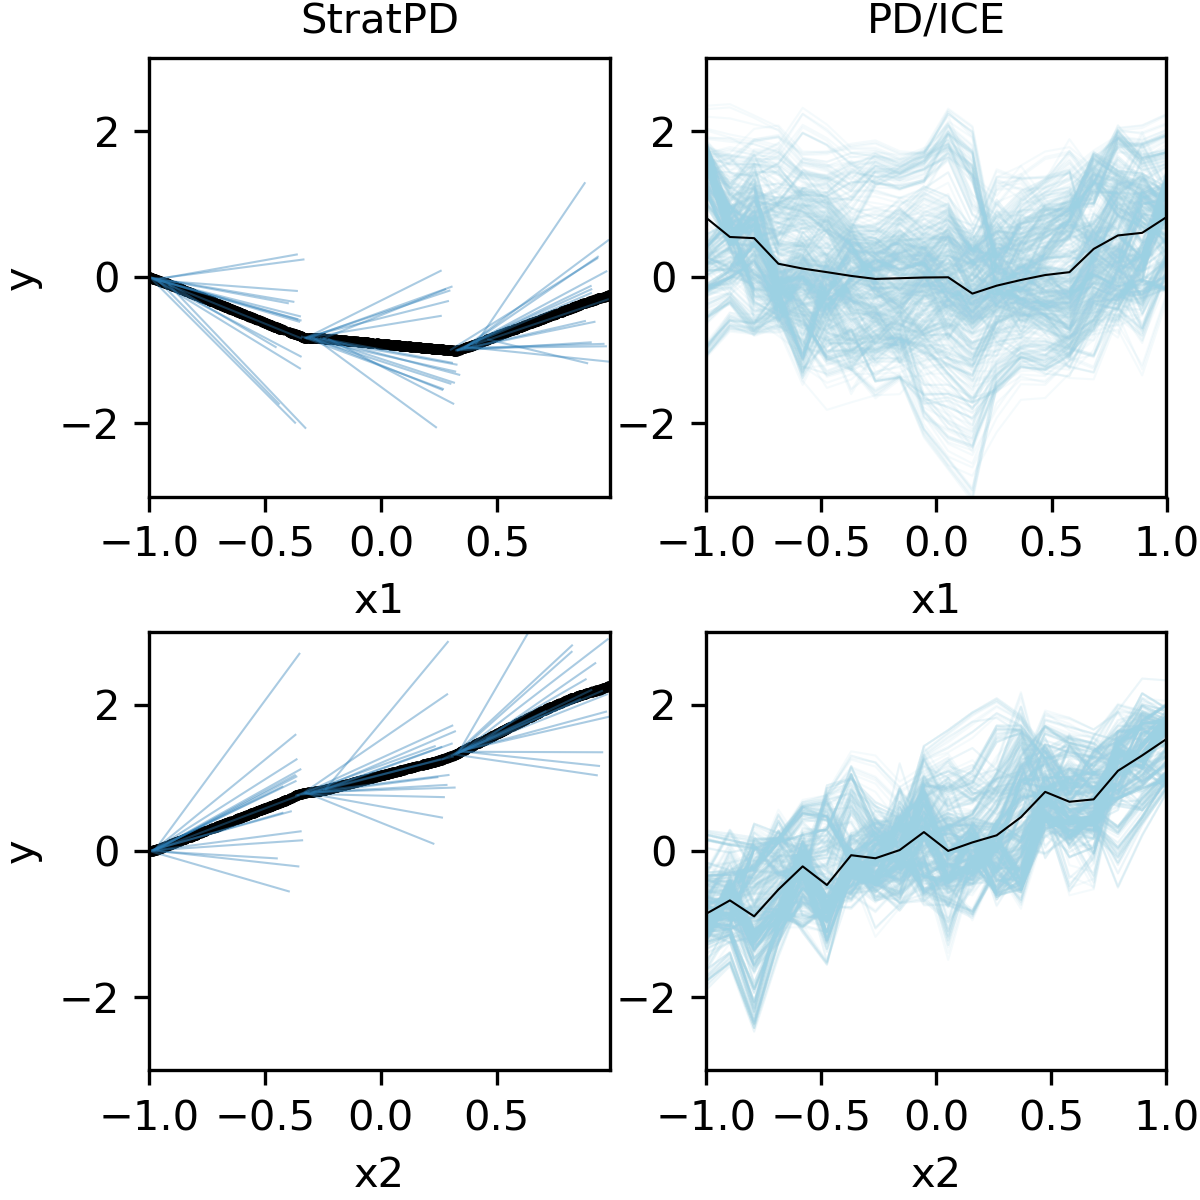
\includegraphics[scale=0.7]{images/additivity.png}
\caption{{\bf big X from ICE, additivity from PD/ICE}}
\label{fig:bigx_y_stratpd}
\end{center}
\end{figure}

\begin{figure}[htbp]
\begin{center}
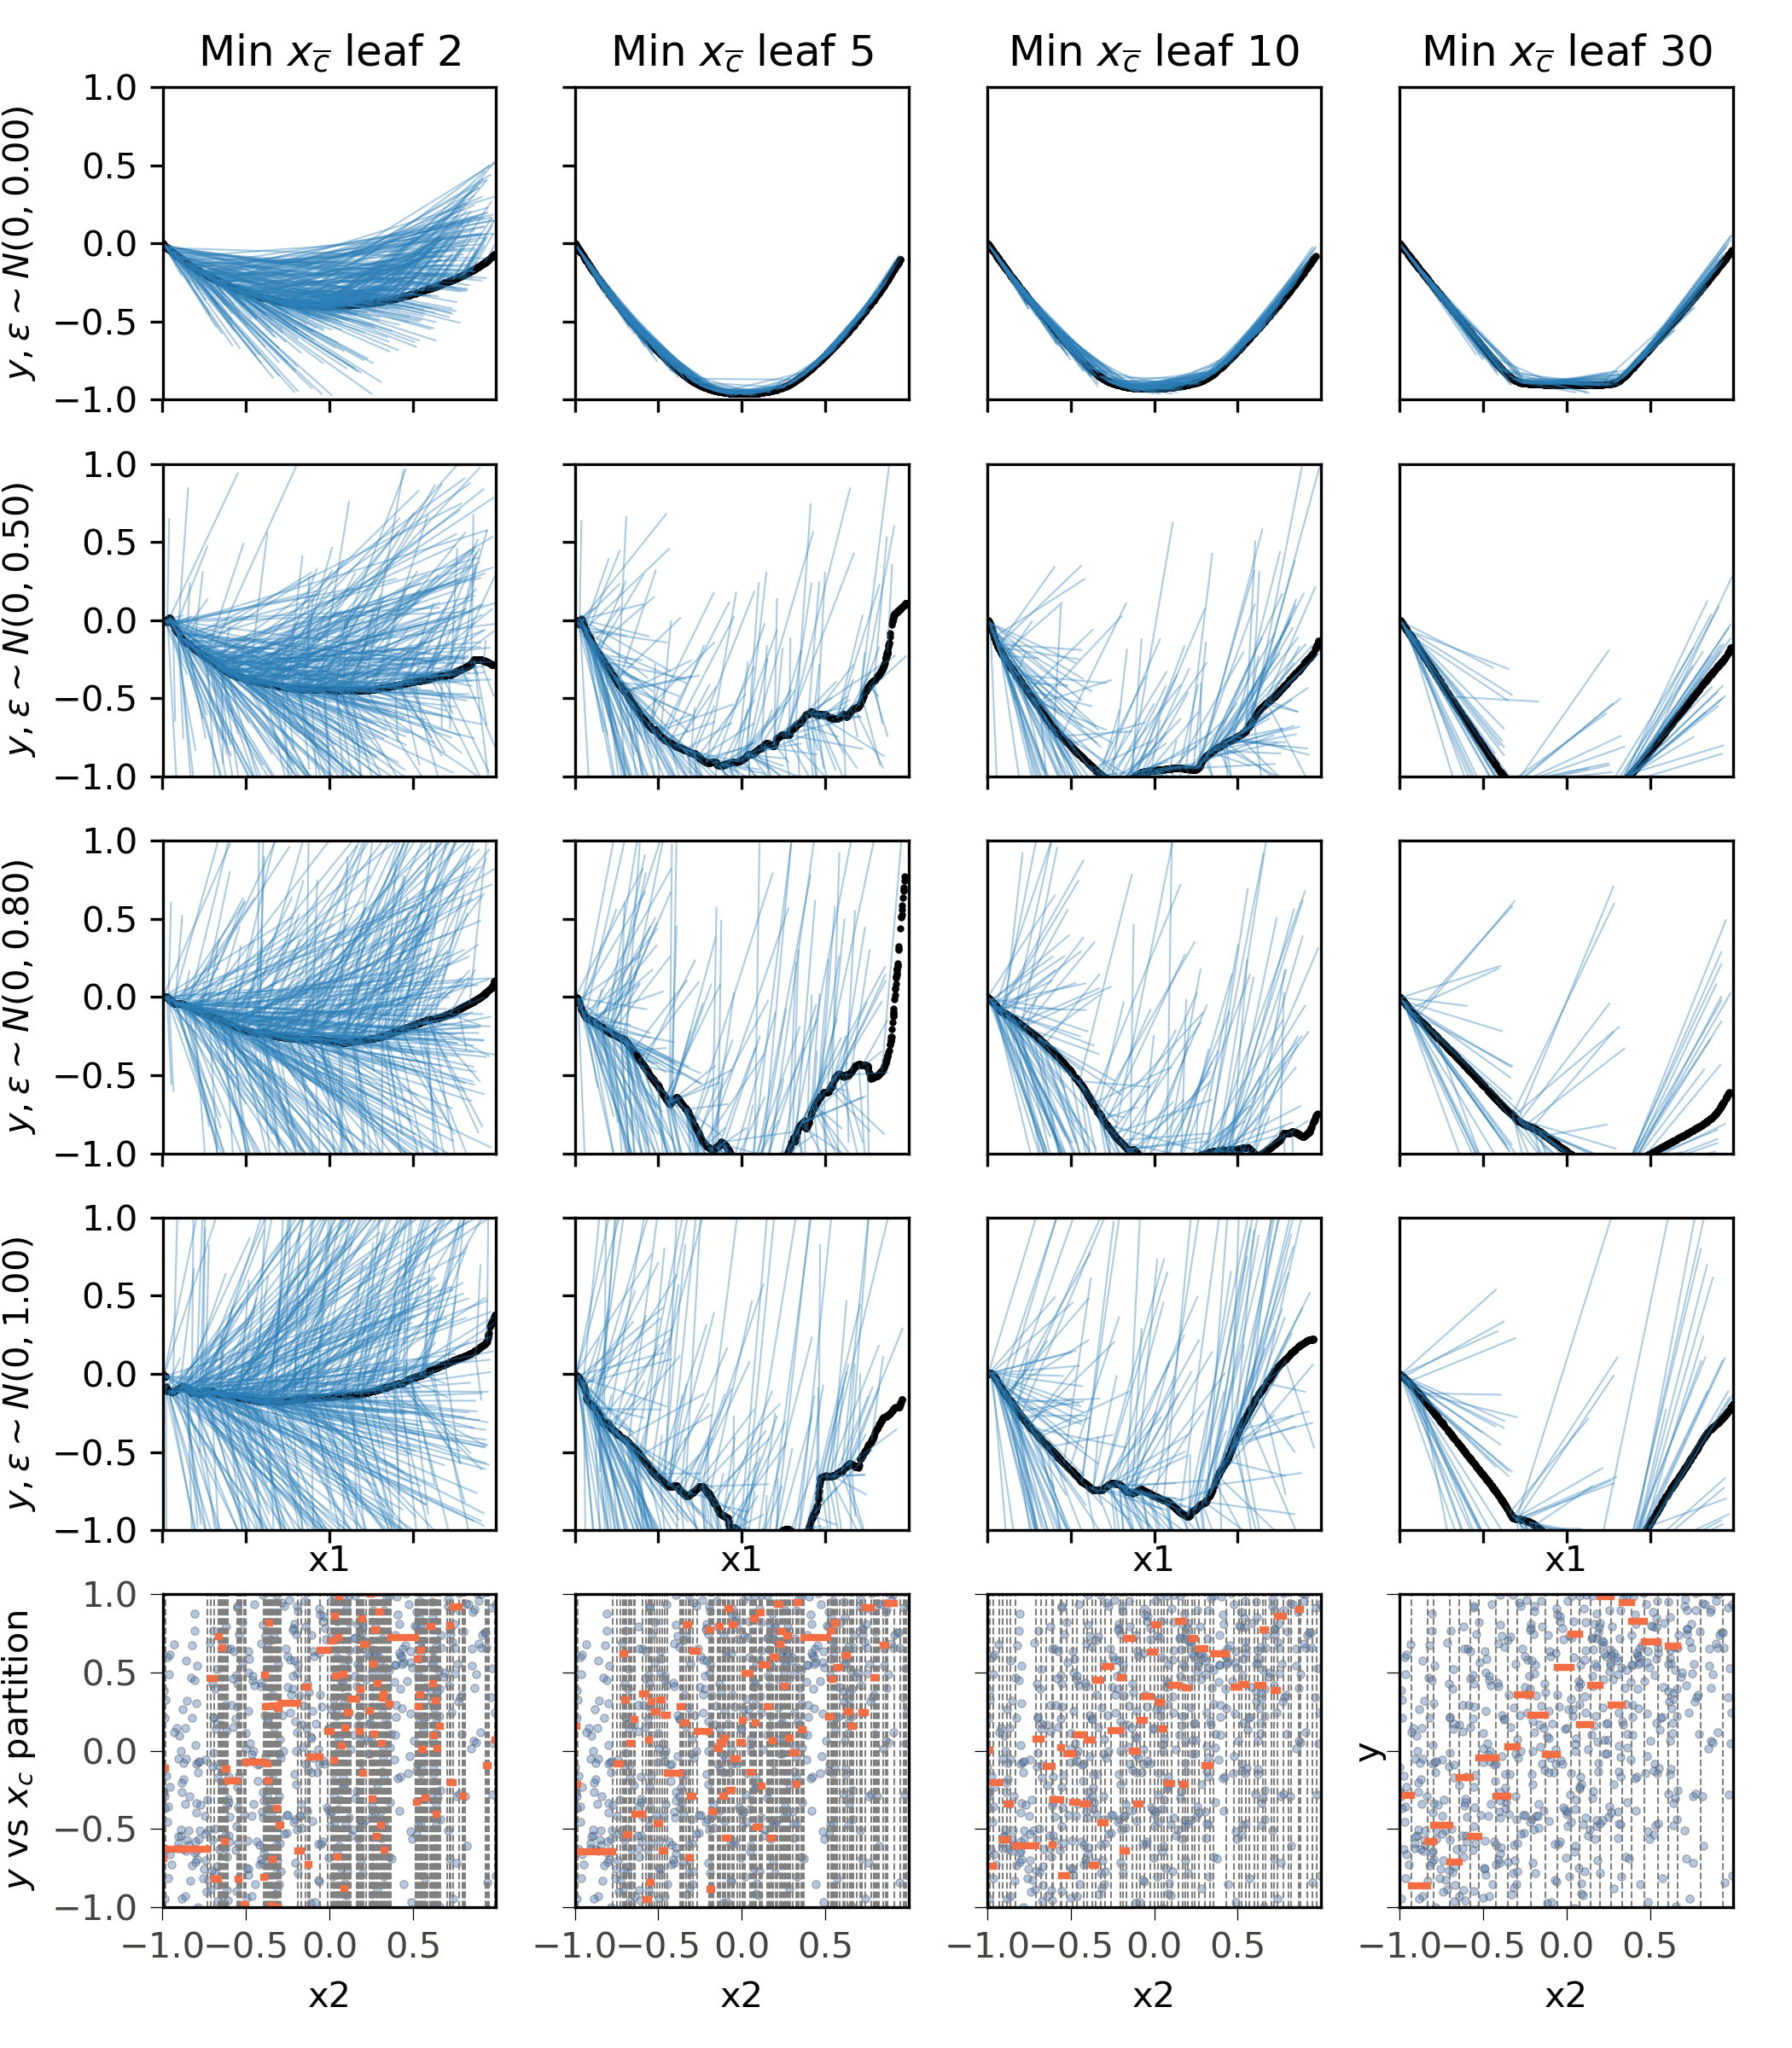
\includegraphics[scale=0.7]{images/meta_additivity_noise.png}
\caption{effect of noise}
\label{fig:meta_noise}
\end{center}
\end{figure}

\begin{figure}[htbp]
\begin{center}
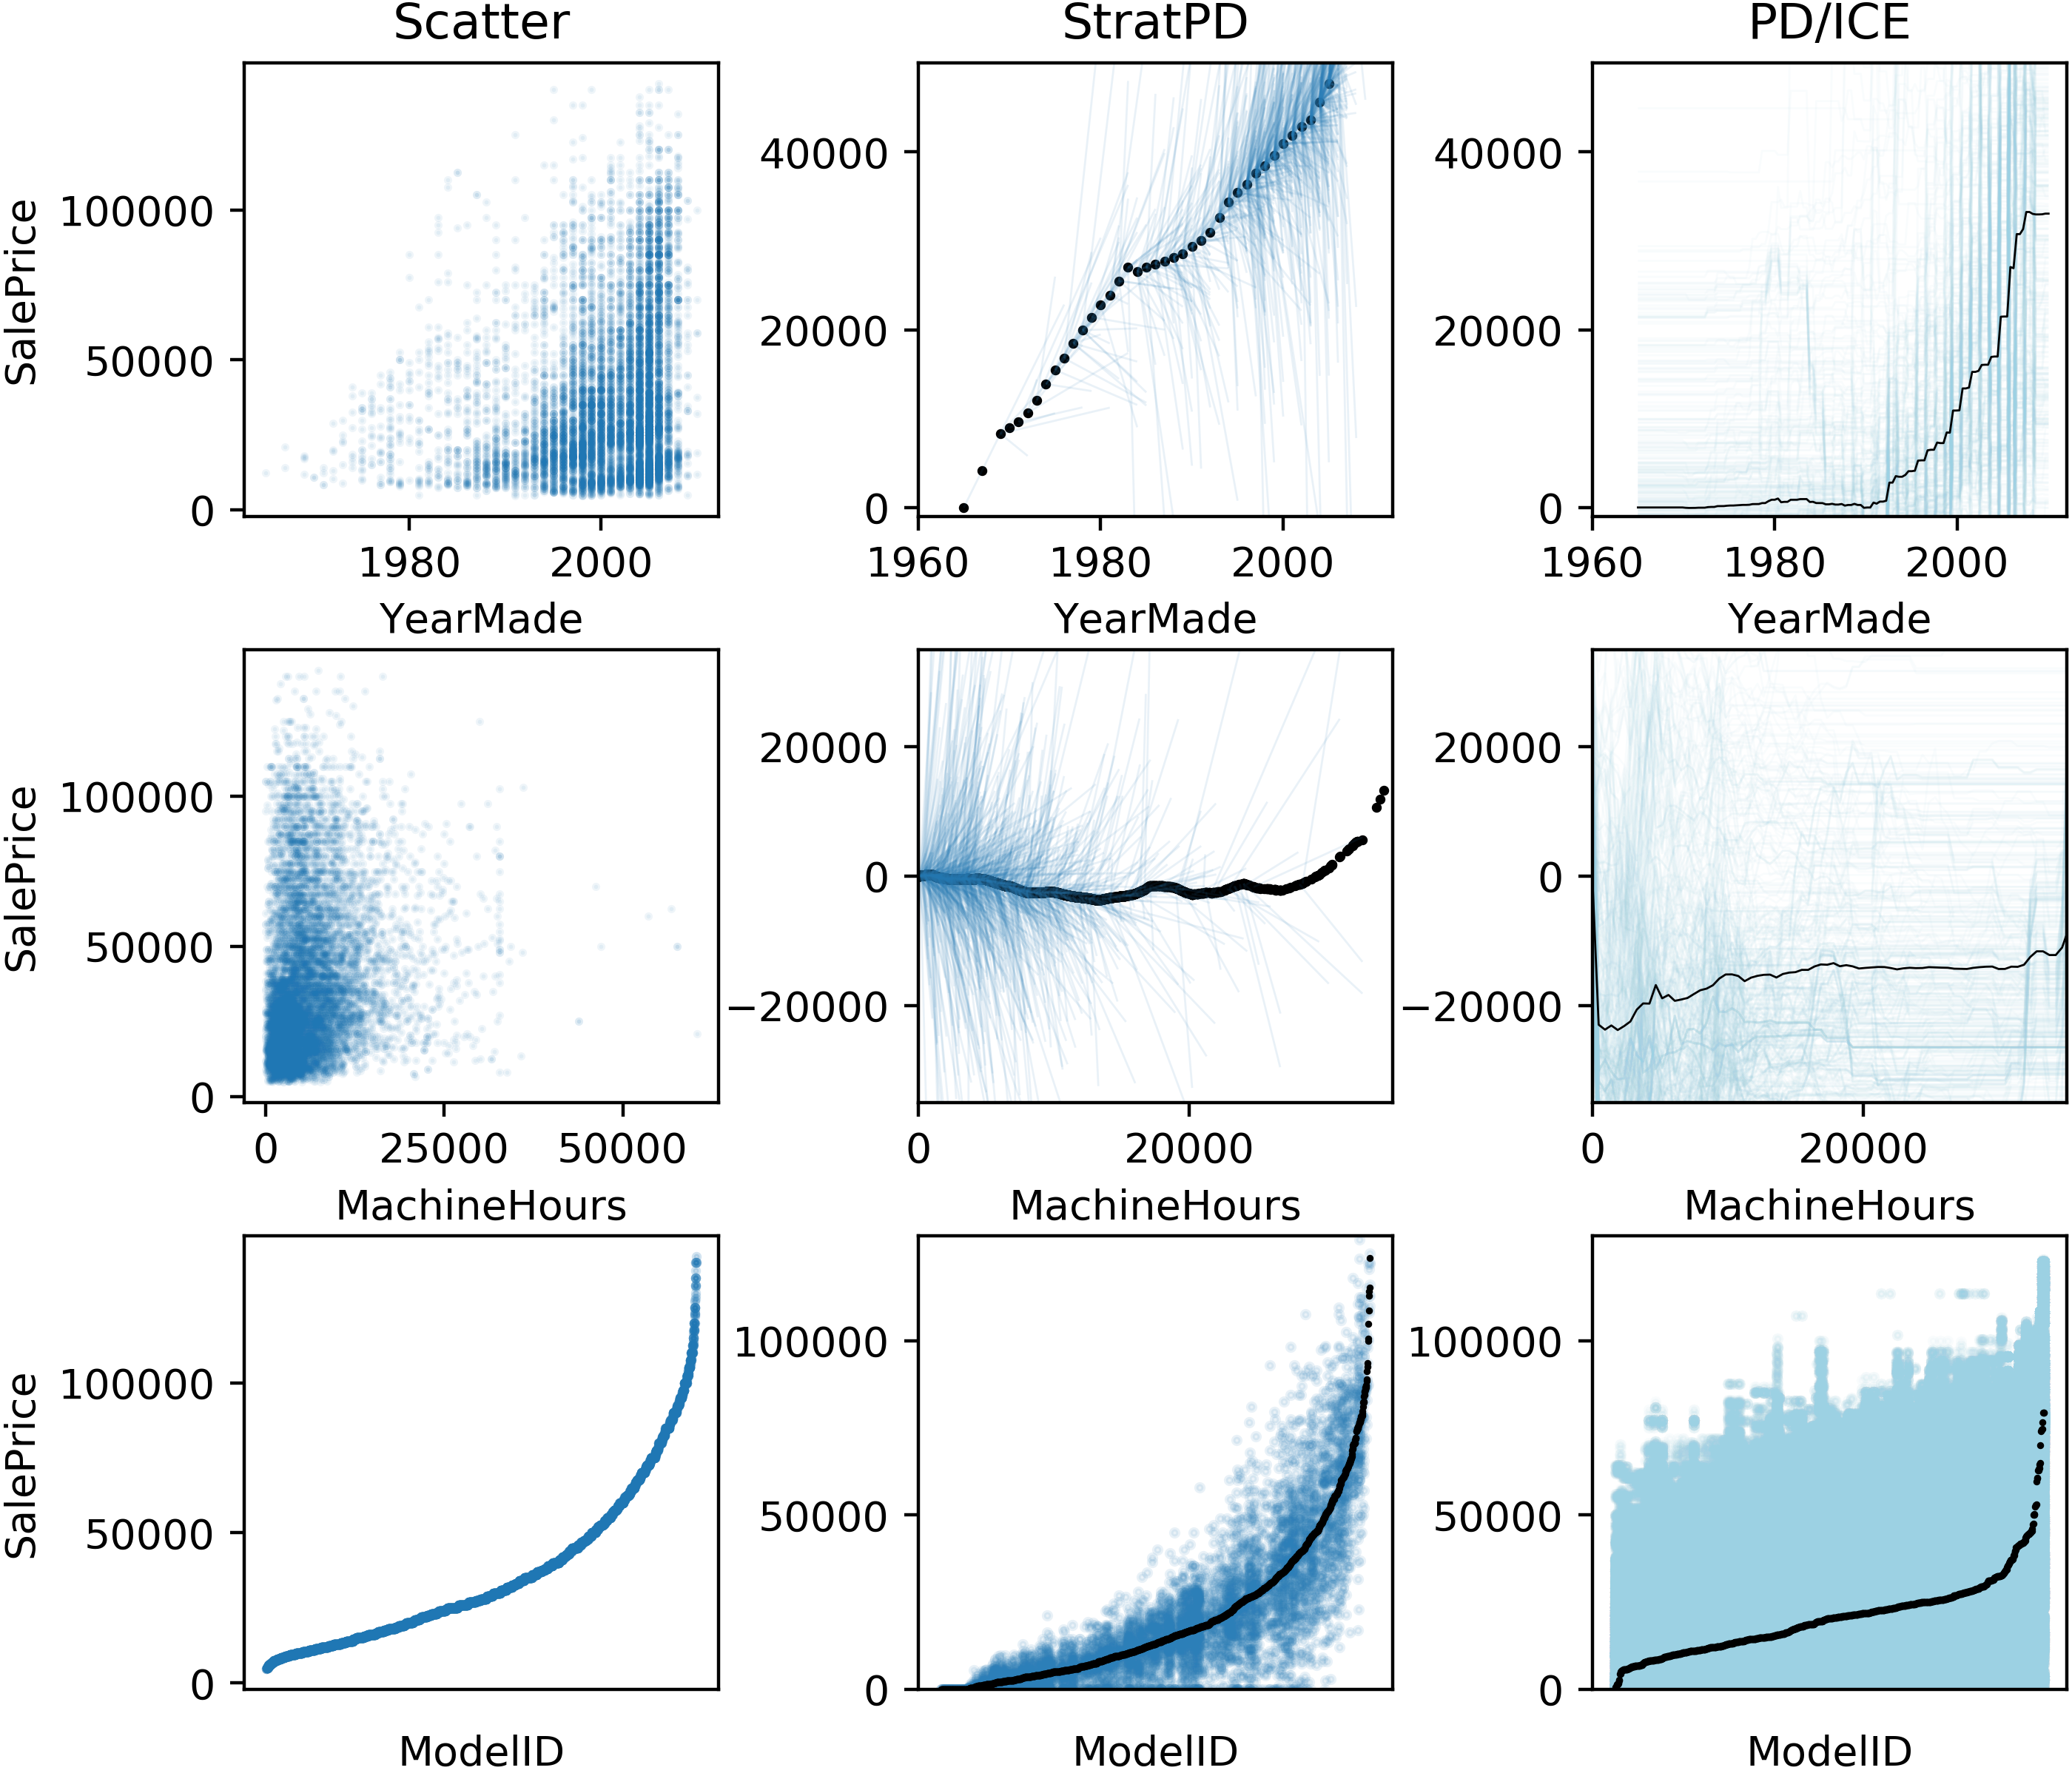
\includegraphics[scale=0.7]{images/bulldozer.png}
\caption{bulldozer; endogeneity}
\label{fig:bulldozer}
\end{center}
\end{figure}

\begin{figure}[htbp]
\begin{center}
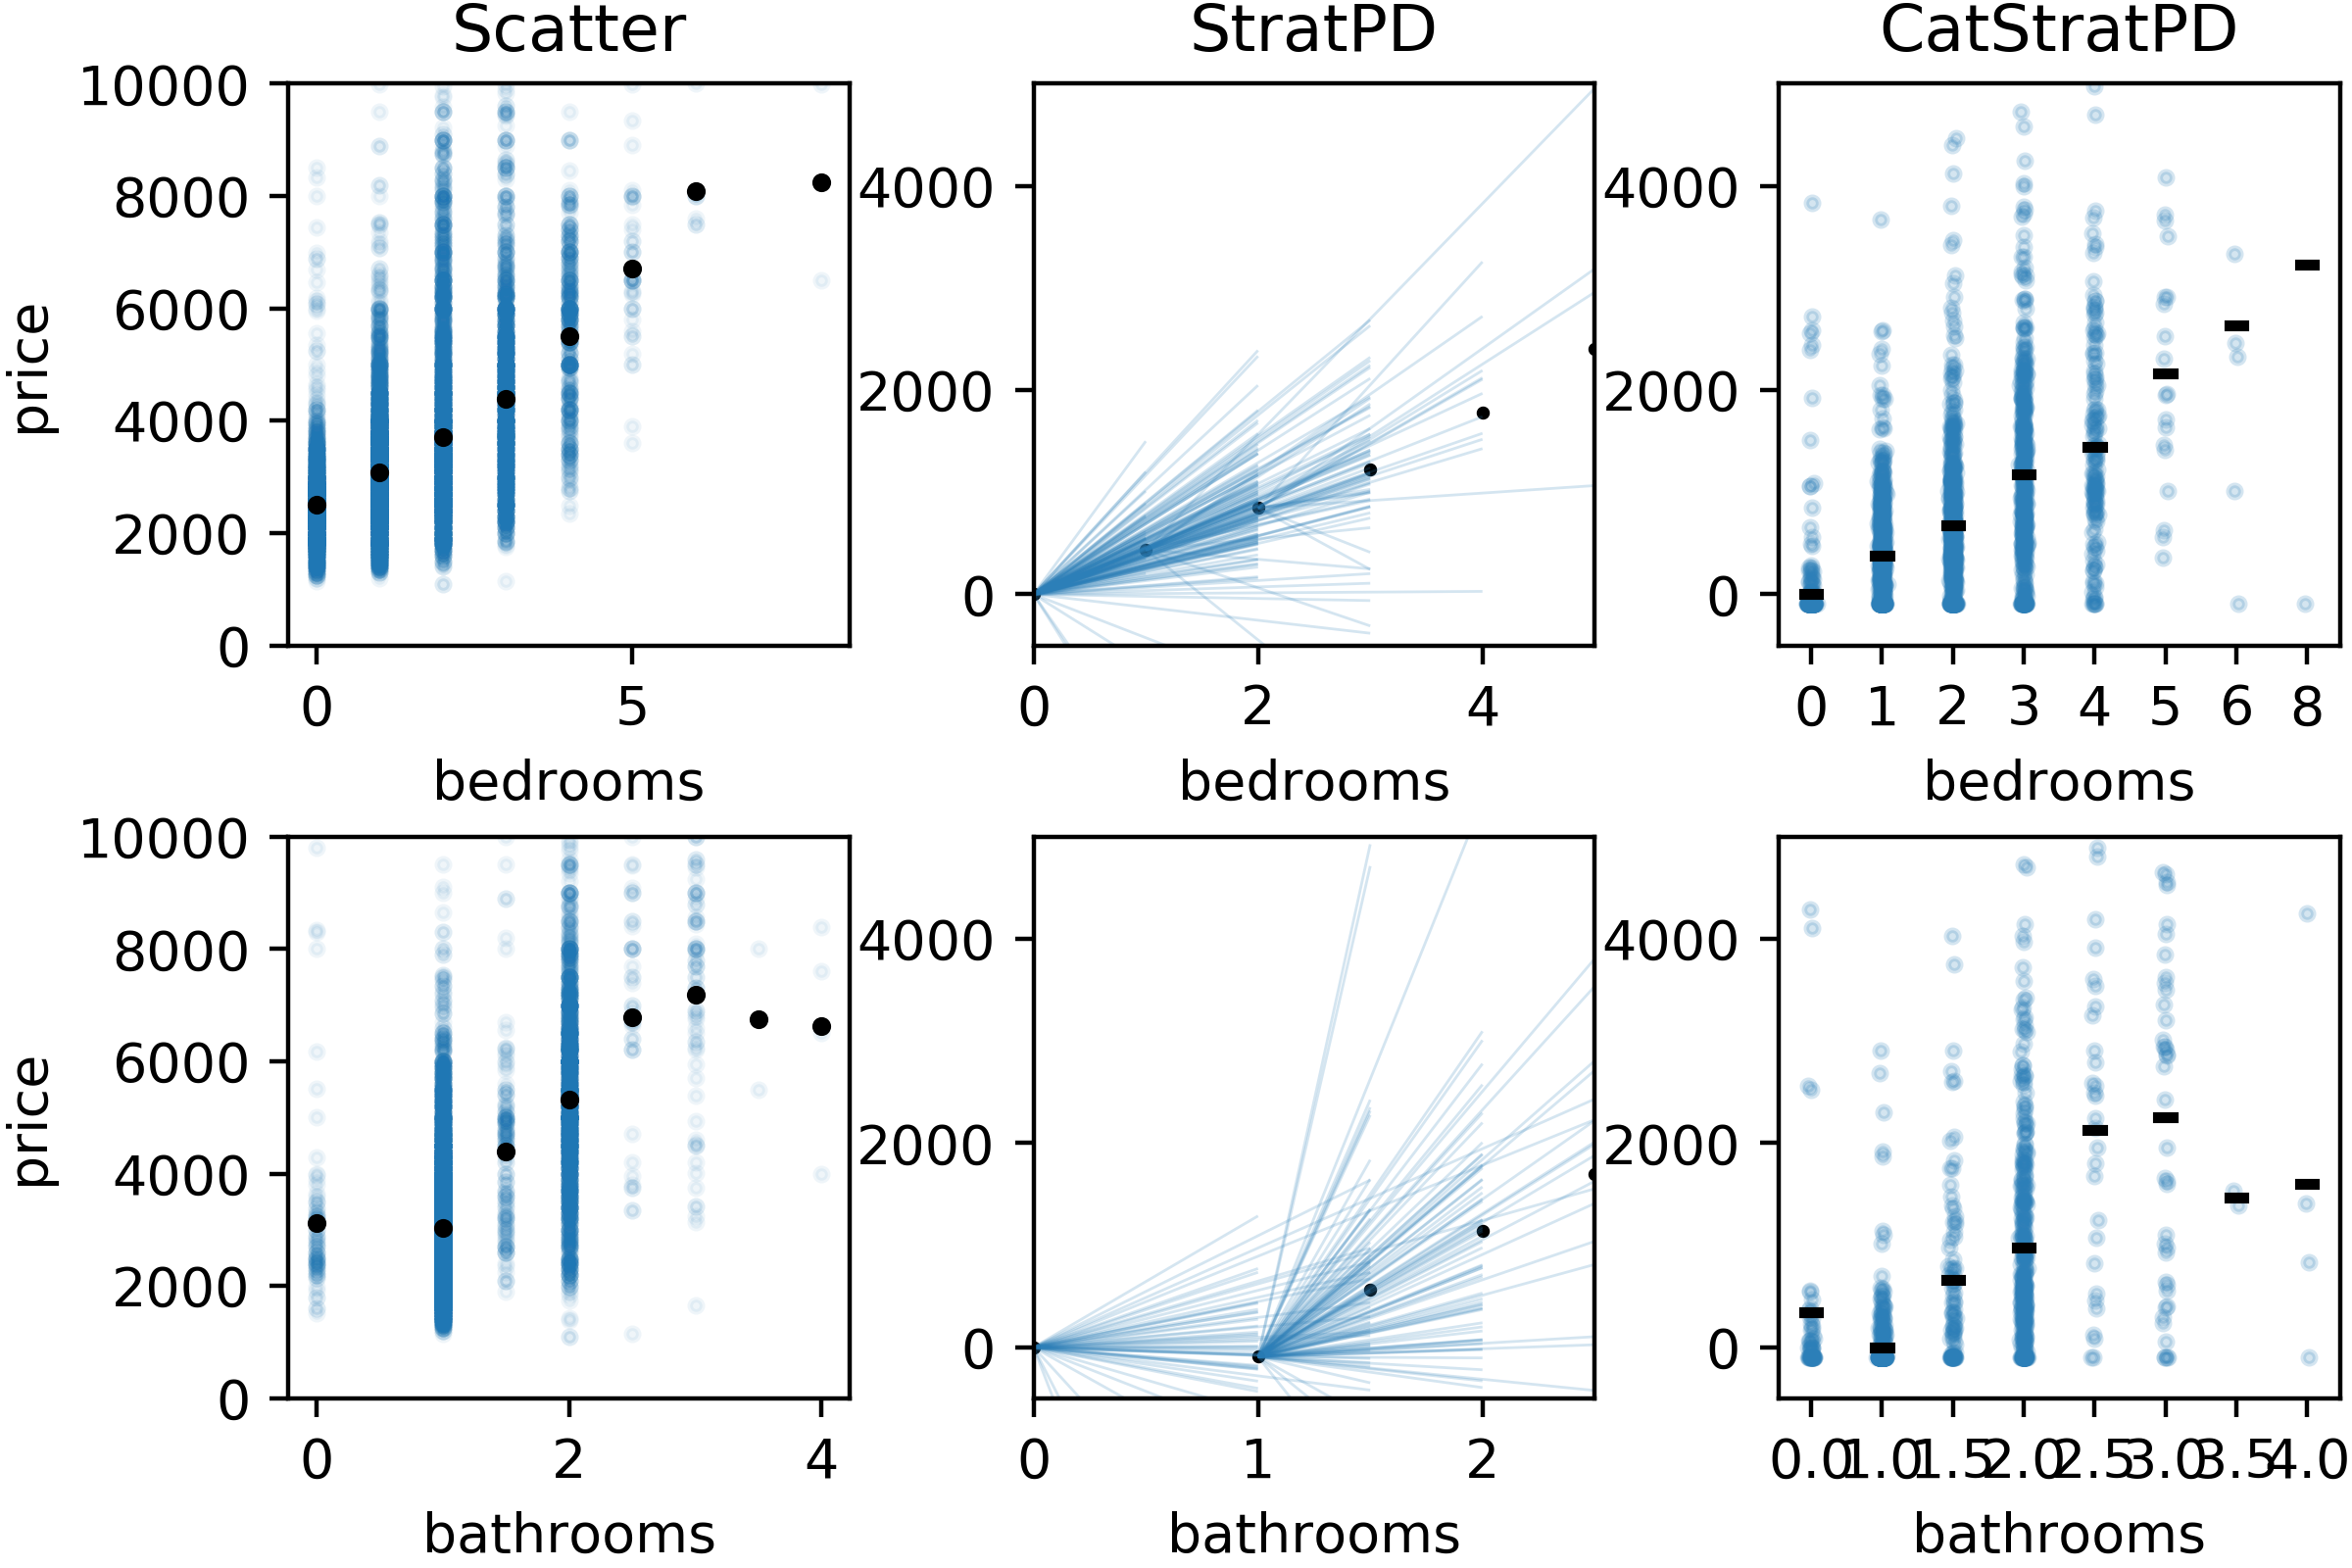
\includegraphics[scale=0.7]{images/rent_intcat.png}
\caption{int cat not usual stratpd}
\label{fig:rent_intcat}
\end{center}
\end{figure}


\subsection{Approximating partial derivatives for large regions}\label{sec:patho}

There is a pathological case to consider where training yields a decision tree with very large leaves, with perhaps hundreds or thousands of observations.  This can happen when \xnc{} contains a single categorical variable or when the only strongly-predictive variable in \xnc{} is categorical.  Training a single linear model through hundreds of $(Lx, Ly)$ observations is unlikely to capture the relationship.  The weather data set is a case in point. Choosing $x_c$=$x_{dayofyear}$, leaves \xnc{}=\{$x_{state}$,$x_{year}$\} and $x_{state}$ accounts for most of the variation in target variable temperature.  \figref{fig:dayofyear_vs_temp}(a) shows the marginal plot of $x_{state}$ versus temperature. A decision tree, $T$, splitting on just state, would group all 365 daily temperature observations for a single state into just one leaf. (The marginal plot is showing the complete sine waves but from the side, edge on.)  The \spd{} algorithm described so far would likely create just four linear models, one per state, and would fail to capture the sine waves. PD and ICE plots, on the other hand, identify the noisy sine waves, as shown in \figref{fig:dayofyear_vs_temp}(b). \todo{uses random forest with how many trees for pd/ice?}

To handle the special case where partitioning feature space \xnc{} yields a leaf, $L \in T$, with too many $x_c$ observations, \spd{} trains another decision tree, $T'$, to partition $L$'s $x_c$ space in more detail. In the worst case, every region of \xnc{} identified by $T$ is too large and \spd{} must create a new decision tree per $L \in T$. \algref{alg:StratPD} (lines 6-9) engages this mechanism when $|L|$ is greater than a threshold (default is 30 observations). The \spd{} plot in \figref{fig:dayofyear_vs_temp}(c) clearly shows the sinusoidal temperature fluctuations over the year. The PD/ICE plot is not smooth because it relies on predictions from a model trained on noisy data, whereas the \spd{} plot is averaging slopes that are themselves smoothing agents.

Without this special case mechanism, the \spd{} plot would have to approximate an entire sine wave with a single line.  Unfortunately, we had to manually choose a suitable minimum leaf size for the nested leaf partitioning, $T'$, to reveal a proper sine wave.  We recommend trying $T'$ multiple minimum leaf sizes for \spd{} plots when \xnc{} has categorical variables and $p$ is small. (The Python implementation allows programmers to set the minimum leaf size for both the \xnc{} partitioning with $T$ and second stage partitioning with $T'$.)

\begin{figure}[htbp]
\begin{center}
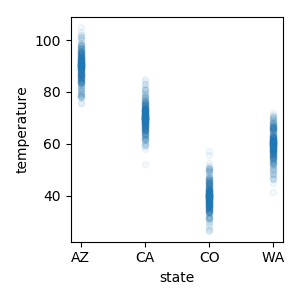
\includegraphics[scale=0.7]{images/state_vs_temp.png}
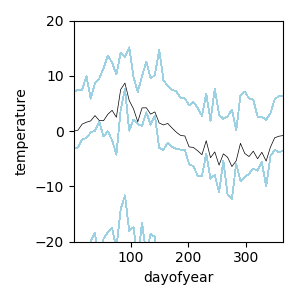
\includegraphics[scale=0.7]{images/dayofyear_vs_temp_pdp.png}
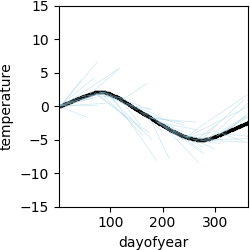
\includegraphics[scale=0.7]{images/dayofyear_vs_temp_stratpd.png}
\caption{{\bf  dayofyear  vs temp}}
\label{fig:dayofyear_vs_temp}
\end{center}
\end{figure}

As another example, compare the PD/ICE (c) and \spd{} (d) plots in \figref{fig:education_vs_weight} showing number of years of education versus weight using the same data set. Weight is related to education by slope -1.2 so a perfect partial dependence graph would show a drop of 12 pounds over 10 years of education.   The PD/ICE plot captures only about half of that relationship, whereas, the \spd{} plot gets much closer to the true education-weight relationship. Female observations have at least 12 years of education, versus 10 for males, so $x_{education}$ and $x_{sex}$ are codependent, though, there is no interaction term. The fact that women are shorter on average biases the education-weight PD/ICE plot because the baseline weight is lower from which the education contribution is  subtracted.

\begin{figure}[htbp]
\begin{center}
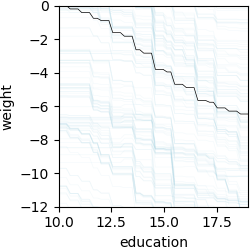
\includegraphics[scale=0.7]{images/education_vs_weight_pdp.png}
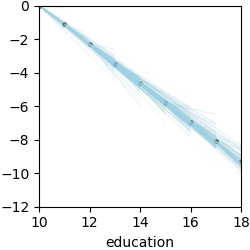
\includegraphics[scale=0.7]{images/education_vs_weight_stratpd.png}
\caption{{\bf  educ vs weight}}
\label{fig:education_vs_weight}
\end{center}
\end{figure}

When there is little codependence between features, the PD and ICE plots represent the partial dependencies well, as is the case with the well-known mtcars data set from \cite{mtcars}, shown in the second column of \figref{fig:cars}.  The first column represents the traditional marginal plots of horsepower and weight to mpg (miles per gallon). The third column represents the \spd{} plots. The orange line in each row represents the regression coefficient of the associated feature (with $y$-intercept adjusted so the line coincides well with the ICE and \spd{} plot slopes).  While both approaches yield useful graphs, the \spd{} plots are smoother and visually appear to be more linear, giving a better fits to the slope lines.

\todo{CARS: edges/outliers of weight and hp not valid as nonsensical values; smoother. clearly nonlinear physics.

\begin{figure}[htbp]
\begin{center}
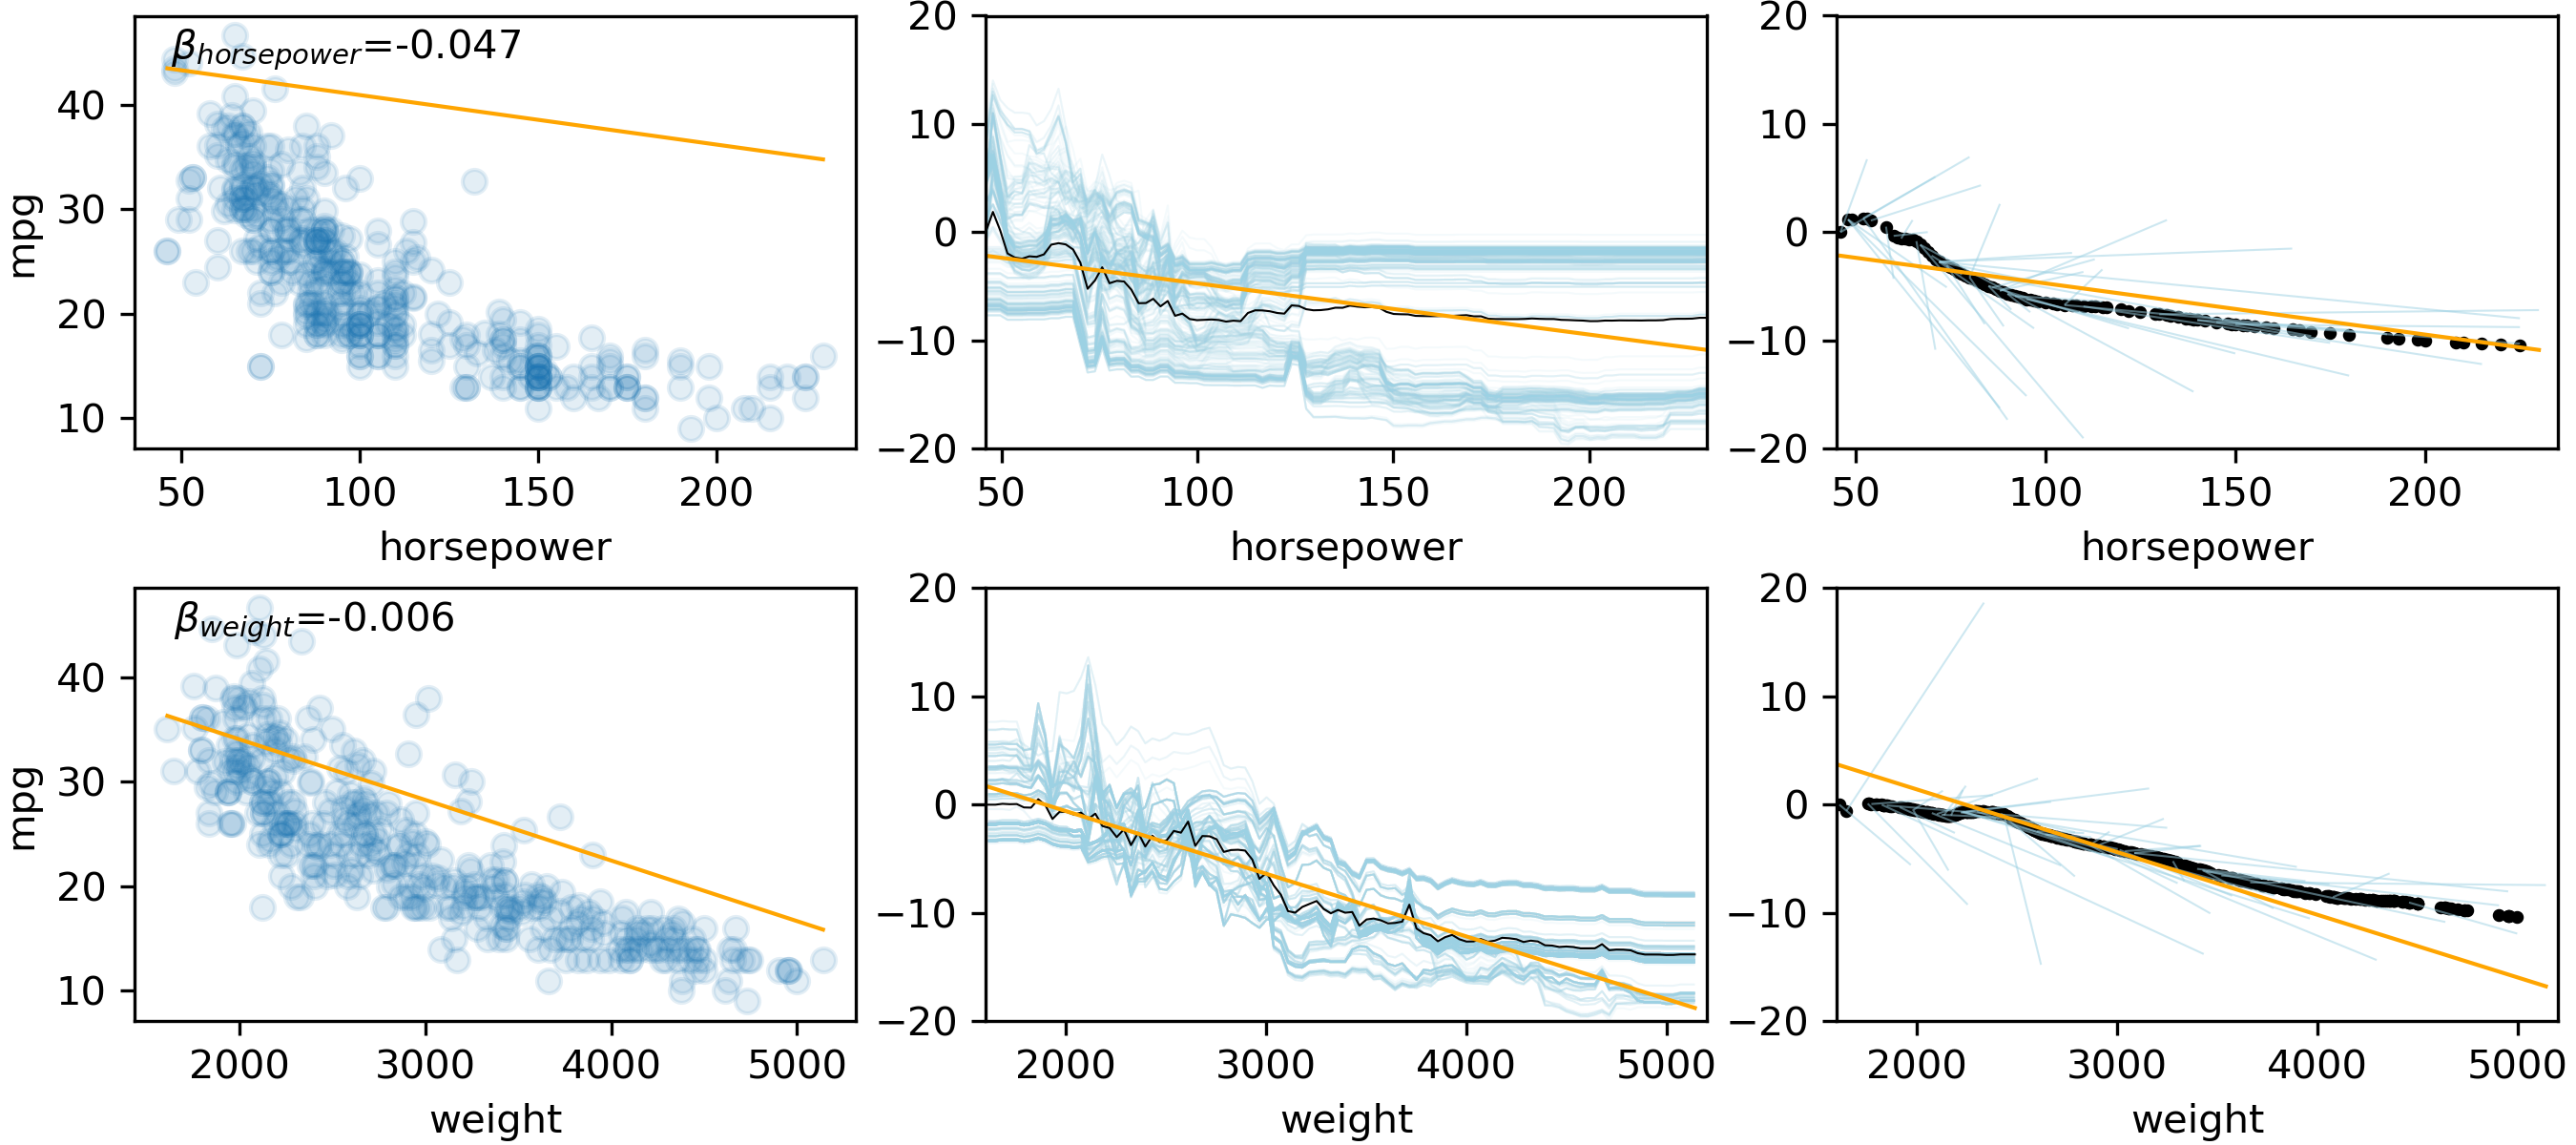
\includegraphics[scale=0.7]{images/cars.png}
\caption{{\bf  cars}}
\label{fig:cars}
\end{center}
\end{figure}

noisy $\sigma^2 = 1.0$ additivity. adding bootstrap trees had no effect on $x_1^2$.  to defeat super noisy stuff we have to increase the number of samples per leaf for $T$ and $T'$; min\_samples\_leaf=30, min\_samples\_leaf\_hires=.4 seems pretty good.  leaving min\_r2 as .5 is fine.  The .4 seems to be a big deal.   adding trees with bootstrapping definitely does not seem to affect anything.  For $x_2$, however, reducing r2 threshold to .1 helps a lot capture slope of two because the linear model is a good approximation to the linear relationship. Leaving r2 at .5 gets a slope of one instead of two. min\_samples\_leaf\_hires doesn't seem important for $x_2$ once we reduce r2 threshold. we also don't have to increase the minimum samples per leaf of T. just the r2 thing makes it work well. the biggest thing is reduce the amount of noise. what is effect or more data but still noisy??? going from 1000 to 2 to 3 to 4000 has no effect; still can't see $x_1^2$ with  default parameters.

similarly, dayofyear vs temperature sine wave does a little better with min\_samples\_leaf=30 due to noise

dup'd column. max curve 2657, max curve with dup 1791 with dup'd bedrooms col.  If i do 20 trees, auto max features, bootstrapping, i get: max curve 2657, max curve with dup 2161. 100 trees: max curve 2657, max curve with dup 2245. ICE for comparison: max ICE curve 2600, max curve with dup 1136. it seems to get hit more! Wow. max\_features=2 and we return to normal with 10 trees: max curve 2657, max curve with dup 2910. Wow. even 2 trees works: max curve 2657, max curve with dup 3039. Turn off bootstrap (2 trees, max feat 2): max curve 2657, max curve with dup 2595. 10 trees, 2 features: max curve 2657, max curve with dup 2623. hooray!  the reason that the ice plot is lowered is due to the data, which has very few data points in the high range of bedrooms. The average is maybe 1.2, so for roughly half the trees, the prediction will be for 1.2 bedrooms no matter what the duplicated bedroom column says.  This problem occurs for strongly predictive features in RF. Linear model couldn't handle duplicate column. \spd{} must use randomness to overcome duplicated columns, but bootstrapping is not important and in fact a negative as we discussed.   tried again with a single max feature and it seems overestimate now:

features = ['bedrooms', 'bathrooms', 'latitude', 'longitude']
max curve 2657, max curve with dup 3509 (10 trees, 1 features, yes bootstrap)
max curve 2657, max curve with dup 3277 (10 trees, 1 features, no bootstrap)
max curve 2657, max curve with dup 2910 (10 trees, 2 features, yes bootstrap)

do the same thing again for bathrooms.
max ICE curve 3257, max curve with dup 1291
max curve 2640, max curve with dup 242 (1 tree)
max curve 2640, max curve with dup 775 (10 trees, 2 features, no bootstrap) more trees doesn't help
max curve 2640, max curve with dup 2220 (10 trees, 1 features, no bootstrap)
max curve 2640, max curve with dup 462 (10 trees, 3 features, no bootstrap)
max curve 2640, max curve with dup 1020 (10 trees, 3 features, yes bootstrap)
max curve 2640, max curve with dup 1142 (10 trees, 2 features, yes bootstrap)
max curve 2640, max curve with dup 2412 (10 trees, 1 features, yes bootstrap)
max curve 2640, max curve with dup 2178 (20 trees, 1 features, yes bootstrap)

Try rent again with noise instead of a duplication column. A single column of noise scaled by 50 dollars does not affect the ice plot (using RF) or the \spd{} plot, as expected.

The data set has an equal number of males and females with $x_{pregnant} \sim U(0,1)$ if female, 65 + $U(-4.5,5)$ if female, and $x_{height} = 68 + U(-7,8)$ if male. 

\[
weight = 120 + 10(x_{height} - min(x_{height})) + 30x_{pregnant} - 1.2x_{education}
\]

$y = 0.2x_1 - 5x_2 + 10x_2\mathbf{1}_{x_3 \geq 0} + \epsilon$, $x_1, x_2, x_3 \in U(-1,1)$, Sample size 1000


\section{Discussion and Future Work}

talk about how, since we don't need y to partition, we can partial out the effects of \xnc{} w/o indirection through fallable model.  We examine $x_c$ relationship with $y$ w/o needing model that fits $X$ to $y$, just $x_c$ to $y$. And locally whereas models tend to optimize globally, leading to potentially high bias on average.

{\color{red} first re-iterate what we did and the main takeaways}. An important feature of \spd{} is that it directly characterizes the relationship between $\mathbf{y}$ and $x_C$ \emph{without} the need for ever training a machine learning model. In this way \spd{} is {model-independent} and will characterize marginal relationships the same way no matter the user's choice of machine learning algorithm. 

This work describes regressors only, ignoring partial dependence for classifiers.  Research reveals no papers or implementation for classifiers. Friedman, however, briefly describes a partial dependence mechanism for classification whereby $k$-class logistic regression (one-versus-rest) equations indicate the probability of seeing class $k$ at $\bf{x}$.  This suffers from the same interaction-based bias as the regressor model.



better handle on hyper parameters; summarize what we know now.

Actually, the R version of personal dependence may actually do this. See https://christophm.github.io/interpretable-ml-book/pdp.html where he describes PDP for cancer prediction and gets probabilities out.

\section{Conclusion}
\label{sec:conc}

\section{Algorithms}

\setlength{\algomargin}{5pt}
\begin{algorithm}[H]
\label{alg:StratPD}
\LinesNumbered
\SetAlgorithmName{Algorithm}{List of Algorithms}
\SetAlgoSkip{}
\SetInd{.5em}{.5em}
\TitleOfAlgo{{\em StratPD}($X$, $\bf y$, $c$, $hires$=30) {\bf returns} collection of $\beta$ coefficients, $\hat{y}$}
Train decision tree regressor $T$ on (\xnc{}, $\bf y$)\\
$leaves$ = leaves($T$)\\
\ForEach{leaf $L \in leaves$}{
	$(Lx, Ly)$ = $\{(x_{ic},  y_i)\}_{i \in L}$\\
	\If{$|L| > hires$}{
		Train decision tree regressor $T'$ on $(Lx, Ly)$\\
		Add leaves($T'$) to $leaves$\\
	}
	$R_L$ = $[min(Lx), max(Lx)]$\\
	\lIf{left$(R_L)$ = right$(R_r)$}{{\bf continue}}\\
	Fit linear model to $(Lx, Ly)$ giving $\beta_L$\\
}
$uniqx$ = sorted(unique($x_c$))\\
\For{$i=1$ {\bf to} $|uniqx|-1$}{
	$R$ = $(uniqx_i, uniqx_{i+1})$\\
	\ForEach{leaf $L \in leaves$}{
		$\beta_{R} = \frac{1}{|R_L \in R|}\Sigma_{R_L \in R}\beta_L$\\
	}
}
$\hat{y}$ = numerically integrate $\beta_R$'s at $uniqx$\\
\Return{collection of all $\beta_R$ and $\hat{y}$}
\end{algorithm}

\setlength{\algomargin}{5pt}
\begin{algorithm}[H]
\label{alg:CatStratPD}
\LinesNumbered
\SetAlgorithmName{Algorithm}{List of Algorithms}
\SetAlgoSkip{}
\SetInd{.5em}{.5em}
\TitleOfAlgo{{\em CatStratPD}($X$, $\bf y$, $c$) {\bf returns} dictionary mapping category to effect on $y$}
Train decision tree regressor $T$ on (\xnc{}, $\bf y$)\\
Let $D$ be dictionary mapping category to $y$ value\\
\ForEach{leaf $L \in T$}{
	$(Lx, Ly)$ = $\{(x_{ic},  y_i)\}_{i \in L}$\\
	\ForEach{$cat \in Lx$}{
		$cat_y$ = $Ly[Lx=cat]$\\
		\lIf{$|cat_y| < 2$}{{\bf continue}}\\
		$cat_{avg}$ = $\frac{1}{|cat_y|} \Sigma cat_y$\\
		$cat_{avg}$ = $cat_{avg} - min(Ly)$\tcp*[r]{\it Strip y contribution from \xnc{}}
		$D_{cat}$ = $D_{cat} + cat_{avg}$\\
	}
}
Let $n_{cat}$ be number of $cat_{avg}$ added to $D_{cat}$\\
$D_{cat}$ = $D_{cat} / n_{cat}$\tcp*[r]{\it Take weighted average of leaf averages for $cat$}
\Return{$D_{cat}$}
\end{algorithm}

\bibliographystyle{apalike}

\bibliography{stratpd}
\end{document}